\documentclass[11pt]{article}
%\usepackage{natbib,mybigpackage}
%\usepackage{mybigpackage}
\usepackage[sectionbib,square]{natbib}
\usepackage{amsmath}
\usepackage[a4paper]{geometry}
\usepackage{graphicx}
\usepackage{algorithm}
\usepackage{algorithmic}
\usepackage{amsfonts}
\usepackage{program}
\usepackage{listings}
%\usepackage{algpseudocode}
\usepackage{ragged2e}
\usepackage[utf8]{inputenc}
\def\xbf{\mathbf{x}}
\def\zbf{\mathbf{z}}
\def\xibf{\mathbf{\xi}}
\begin{document}
\begin{enumerate}
\item[\textbf{Q1:}]
\textbf{ To show that if F is Weibull/log normal cumulative distribution \\function ,then for any $\lambda$ such that $-1\leq\lambda\leq1$,\\
$F^{*}(x)=(1+\lambda)F-\lambda F^2$ ,\\
$F^{*}$ is a cumulative distribution function.}

\item[Ans:]
\end{enumerate}
We know that F is a cumulative distribution function on a probability space $(\Omega,A,P)$ if:\\
$F(x)=P(X^{-1}(-\infty,x])$=$P({\omega:X(\omega)\leq x})$ for $\forall$ x~$\in\mathbb{R}$.\\\\
\textbf{Some properties of the cumulative distribution function of a random variable:}\\
\begin{enumerate}
\item \emph{F} is monotonically increasing.\\
To show $F(x_{1})\leq F(x_{2})$ if $x_{1} \leq x_{2}.$\\
Since $~(-\infty,x_{1}]\subseteq(-\infty,x_{2}]~$ for $~x_{1}\leq x_{2}~$ , so  $~X^{-1}(-\infty,x_{1}]\subseteq X^{-1}(-\infty,x_{2}]~$.\\
Hence $F(x_{1})=P(X^{-1}(-\infty,x_{1}])~\leq~P(X^{-1}(-\infty,x_{2}])~=~F(x_{2})$\\\\\\
\item \emph{F} is right continuous, that is $lim_{t\to x_{t>x}}F(t)=F(x+)$.\\
Let us denote $lim_{t\to x_{t>x}}F(t)=F(x+)$\\
Let $A_{n}={\{\omega:X(\omega)\leq x+\frac1n}\}~=~X^{-1}(-\infty,x+\frac1n]$.\\
Then $A_{1}\supseteq A_{2}\supseteq A_{3}\supseteq .........A_{n}\supseteq A_{n+1}.....$\\
So $A_{n}$  is a sequence of contracting (decreasing) events.\\
By the continuity theorem\\
$lim_{n\to\infty}F(x+\frac1n)=lim_{n\to\infty}P(A_{n})=P(\cap_{n=1}^\infty A_{n})$\\
$=P(\cap_{n=1}^\infty X^{-1}(-\infty,x+\frac1n] )=P(X^{-1}(\cap_{n=1}^\infty (-\infty,x+\frac1n]))=P(X^{-1}(-\infty,x])=F(x)$\\
Since F is a monotonically increasing function on R, hence $F(x+)$ exists $\forall$ x $\in \mathbb{R}$ and is
finite (since F is bounded) for every real x,\\
so F(x+) = $lim_{n \to\infty}F(x+\frac1n)=F(x)$\\\\
\item $F(-\infty)=lim_{x \to {-\infty}}F(x)=0$\\
Let $A_{n}={\{\omega:X(\omega)\leq -n}\}~=~X^{-1}(-\infty,-n]$.\\
Then $A_{1}\supseteq A_{2}\supseteq A_{3}\supseteq .........A_{n}\supseteq A_{n+1}.....$\\ is a sequence of contracting (decreasing) events.\\
Since F is a bounded, monotonically increasing function $lim_{x \to {-\infty}}F(x)$ exists and $F(-\infty)=lim_{n \to {\infty}}F(-n)=lim_{n \to {\infty}}P(A_{n})=P(\cap_{n=1}^\infty A_{n})=P(\cap_{n=1}^\infty X^{-1}(-\infty,-n] )=P(X^{-1}(\cap_{n=1}^\infty (-\infty,-n]))=P(X^{-1}(\phi))=0$\\\\
\item $F(\infty)=lim_{x \to {\infty}}F(x)=1$\\
Let $A_{n}={\{\omega:X(\omega)\leq n}\}~=~X^{-1}(-\infty,n]$.\\
Then $A_{1}\subseteq A_{2}\subseteq A_{3}\subseteq .........A_{n}\subseteq A_{n+1}.....$\\ is a sequence of increasing events.\\
Since F is a bounded, monotonically increasing function $lim_{x \to {-\infty}}F(x)$ exists and $F(\infty)=lim_{n \to {\infty}}F(n)=lim_{n \to {\infty}}P(A_{n})=P(\cup_{n=1}^\infty A_{n})=P(\cup_{n=1}^\infty X^{-1}(-\infty,n] )=P(X^{-1}(\cup_{n=1}^\infty (-\infty,n]))=P(X^{-1}(\mathbb{R}))=1$\\\\
\end{enumerate}
\textbf{For Weibull Distribution:\\}
$F(x)=1-e^{-\alpha x^{\beta}}~,x>0$\\
\\
$F^{*}(x)=(1+\lambda)F-\lambda F^2$\\
$F^{*}(x)=1+(\lambda -1)e^{-\alpha x^{\beta}}-\lambda e^{-2\alpha x^{\beta}}$\\
\\for property 1,\\
Differentiating $F^{*}(x)$\\
$F^{{*}^{'}}(x)=(1+\lambda)\frac {dF}{dx}-2\lambda F\frac {dF}{dx}$\\
$~~~~~~~~~=(1+\lambda-2\lambda F)\frac {dF}{dx}$\\
Since, F is CDF\\
So,$\frac {dF}{dx}>0$ as F is monotonically increasing.\\
Since,$~~0\leq F \leq 1~~$\\
So,$~0\geq-2\lambda F\geq-2\lambda$\\
So,$~1+\lambda\geq(1+\lambda-2\lambda F)\geq1-\lambda$\\
As, $\lambda\geq-1$,\\
So,$F^{{*}^{'}}(x)>0$\\
Hence, it is monotonically increasing function.\\
\\
for property 2\\
$F^{*}(x+) = lim_{n \to\infty}F^{*}(x+\frac1n)=F^{*}(x)$\\
Now , F is CDF. So , F is right continuous.\\
So, $\lambda F^{2}$ is also right continuous.\\
$(1+\lambda)F-\lambda F^{2}$ will also be a right continuous.\\
\textbf{[Sum of continuous function is also a continuous function.]}\\
Hence, $F^{*}$ is right continuous.\\\\
for property 3,\\
$F^{*}(-\infty)=lim_{x \to {-\infty}}F^{*}(x)=0$\\
Since, F is a CDF\\
So, $F(-\infty)=lim_{x \to {-\infty}}F(x)=0$\\
So,$F^{2}(-\infty)=lim_{x \to {-\infty}}F^{2}(x)=0$\\
So,$(1+\lambda)F(-\infty)-\lambda F^{2}(-\infty)=lim_{x \to {-\infty}}((1+\lambda)F(x)-\lambda F^{2}(x))=0$\\
So,$F^{*}(-\infty)=lim_{x \to {-\infty}}F^{*}(x)=0$\\\\
for property 4\\
$F^{*}(\infty)=lim_{x \to {\infty}}F^{*}(x)=1$\\
Since, F is a CDF\\
So, $F(\infty)=lim_{x \to {\infty}}F(x)=1$\\
So,$F^{2}(\infty)=lim_{x \to {\infty}}F^{2}(x)=1$\\
So,$(1+\lambda)F(\infty)-\lambda F^{2}(\infty)=lim_{x \to {\infty}}((1+\lambda)F(x)-\lambda F^{2}(x))=1+\lambda-\lambda=1$\\\\
So,$F^{*}(\infty)=lim_{x \to {\infty}}F^{*}(x)=1$\\\\
Hence $F^{*}$ follows all four properties of Cumulative Distribution function.\\
So, $F^*$ is a  Cumulative Distribution Function.\\
By inverse transform method:\\
$F^{*}(x)=(1+\lambda)F-\lambda F^{2}=u$ where u $\sim$ U(0,1) \\
So, by solvig the quadratic we get two roots:\\

\[F(x)= \begin{cases} 
      \frac{(1+\lambda)\pm \sqrt{(1+\lambda)^2-4\lambda u}}{2\lambda} & \lambda \neq 0 ,\lambda \in (-1,1) \\\\
      ~~~~~~~~~~~~u & \lambda = 0 \\
      
   \end{cases}
\]\\
Using this we can find out the inverse transformation of $F^{*}(x)$ . For weibull distribution take the root with - sign and for lognormal take the root with + sign as $\forall x \in \mathbb{R}$ we have $F(x) > 0$.\\

\noindent{Code for R}\\
\begin{lstlisting}
\#BY WEIBULL DISTRIBUTION

a<-1
b<-2
d<-c(-1,-0.5,0,0.5,1)
x<-1
j<-1

for(i in 1:5)
{
	while(j<=10000)
	{
		u<-runif(1)
		if(d[i]!=0)
			x[j]=(1/a)*(-1*log(((d[i]-1)+
			 sqrt((1+d[i])^2 - 4*u*d[i]))/(2*d[i])))^(1/b)
		else
			x[j]=(1/a)*(-1*log(1-u))^(1/b)
		j=j+1
	}

	j<-1


	cat("\nThe Mean of the Distributon calculated is ",mean(x))
	cat("\nThe Varinace of the Distributon calculated is ",var(x))
	cat("\n")
	h=ecdf(x)
	plot( h,col="red", xlab="", ylab="Cumulative Distribution",
	 main=paste("\nExperimental CDF of X \nlambda = ",d[i],
	 "\nMean = ",mean(x),"\n Variance = ",var(x))) 
	hist(x,probability='TRUE')
	lines(density(x), col='darkorange')
}
\end{lstlisting}
Here, $\alpha=1,\beta=2$\\\\
\noindent{Histograms:}\newline
\\For $\lambda=-1$\\\\
CDF of X:\\
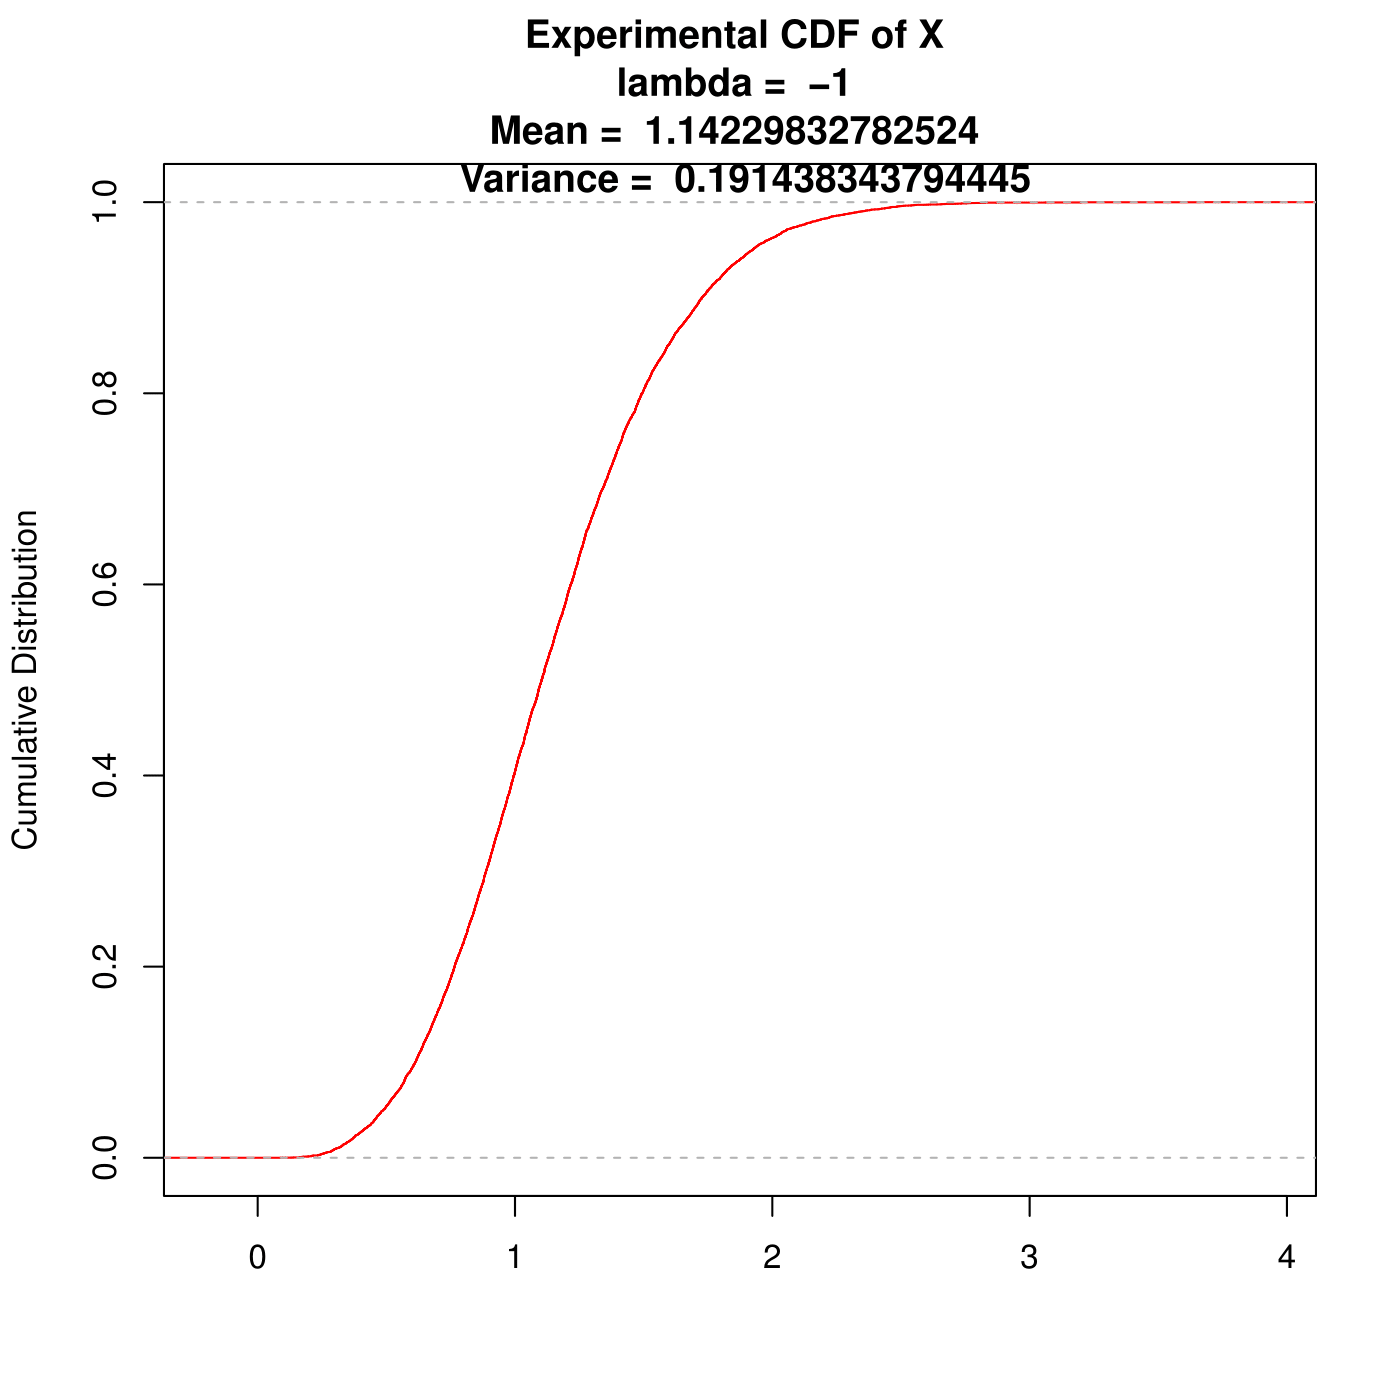
\includegraphics[width=0.90\textwidth]{weibull/Rplots-01.png}{\centering}\\\\
Density of X:\\
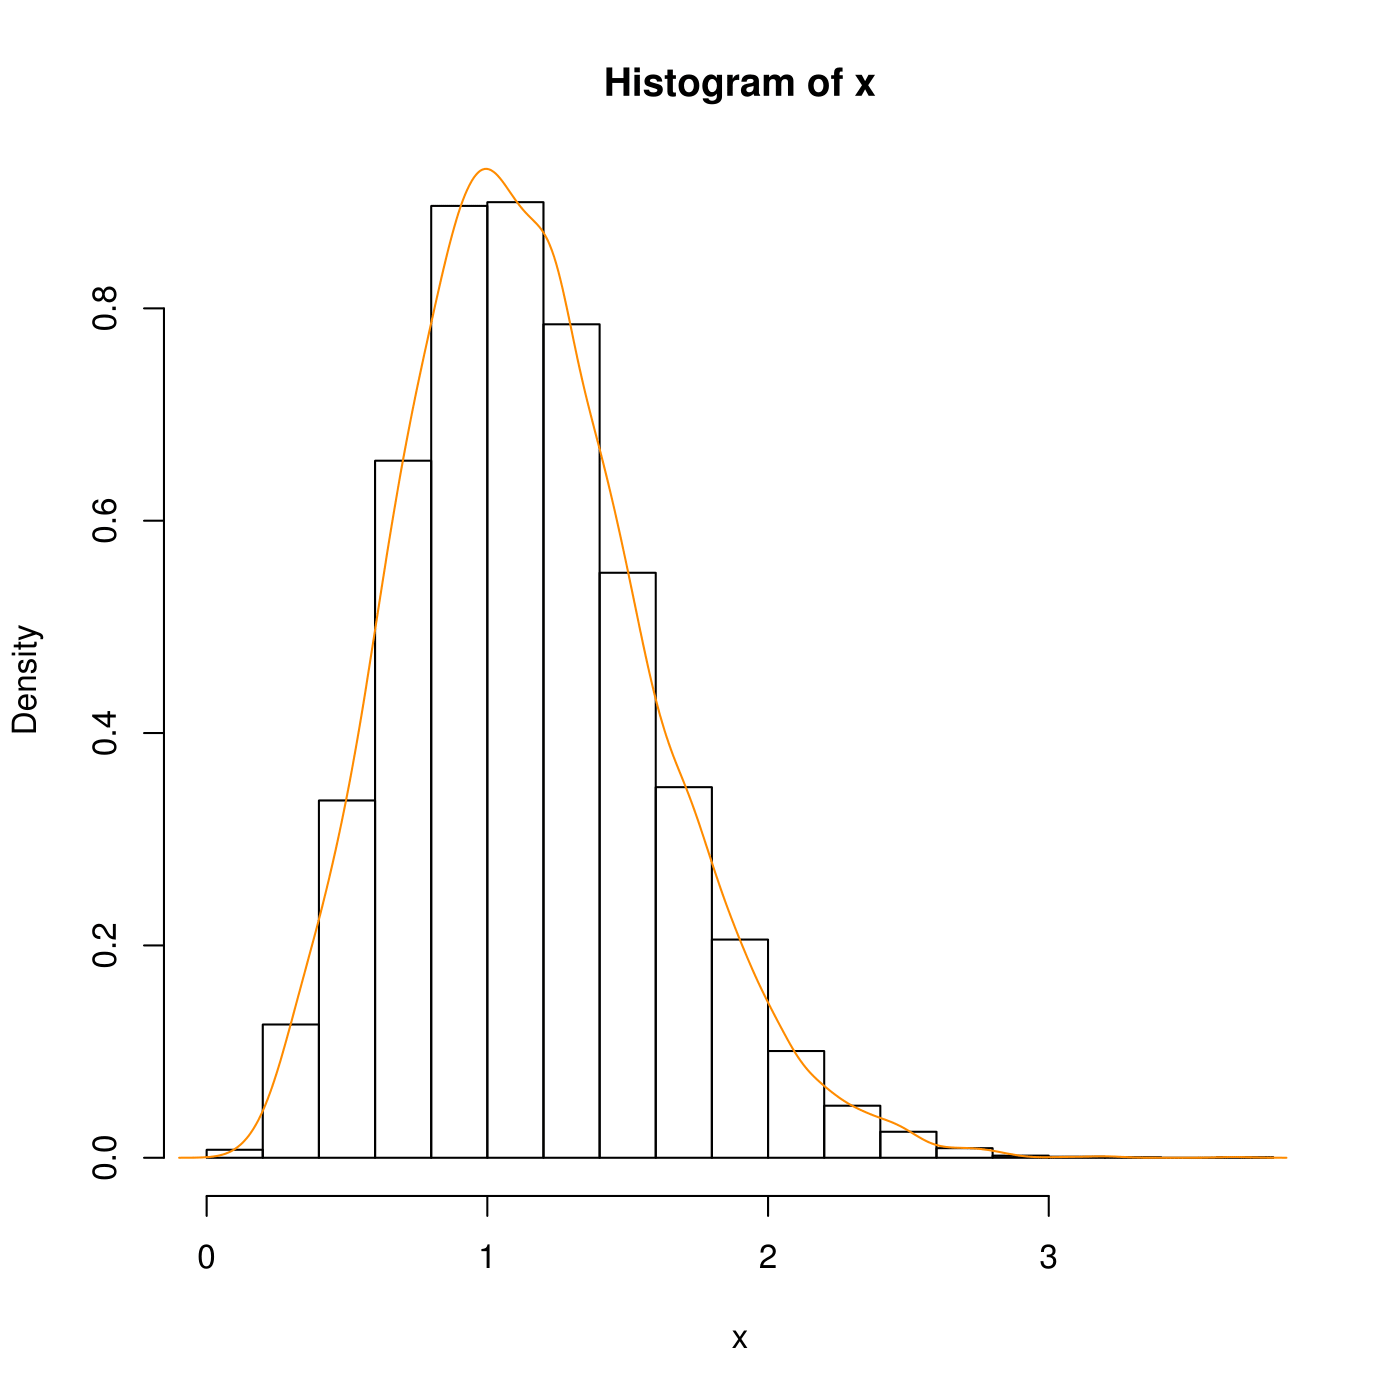
\includegraphics[width=0.90\textwidth]{weibull/Rplots-02.png}{\centering}\\\\
\\For $\lambda=-0.5$\\\\
CDF of X:\\
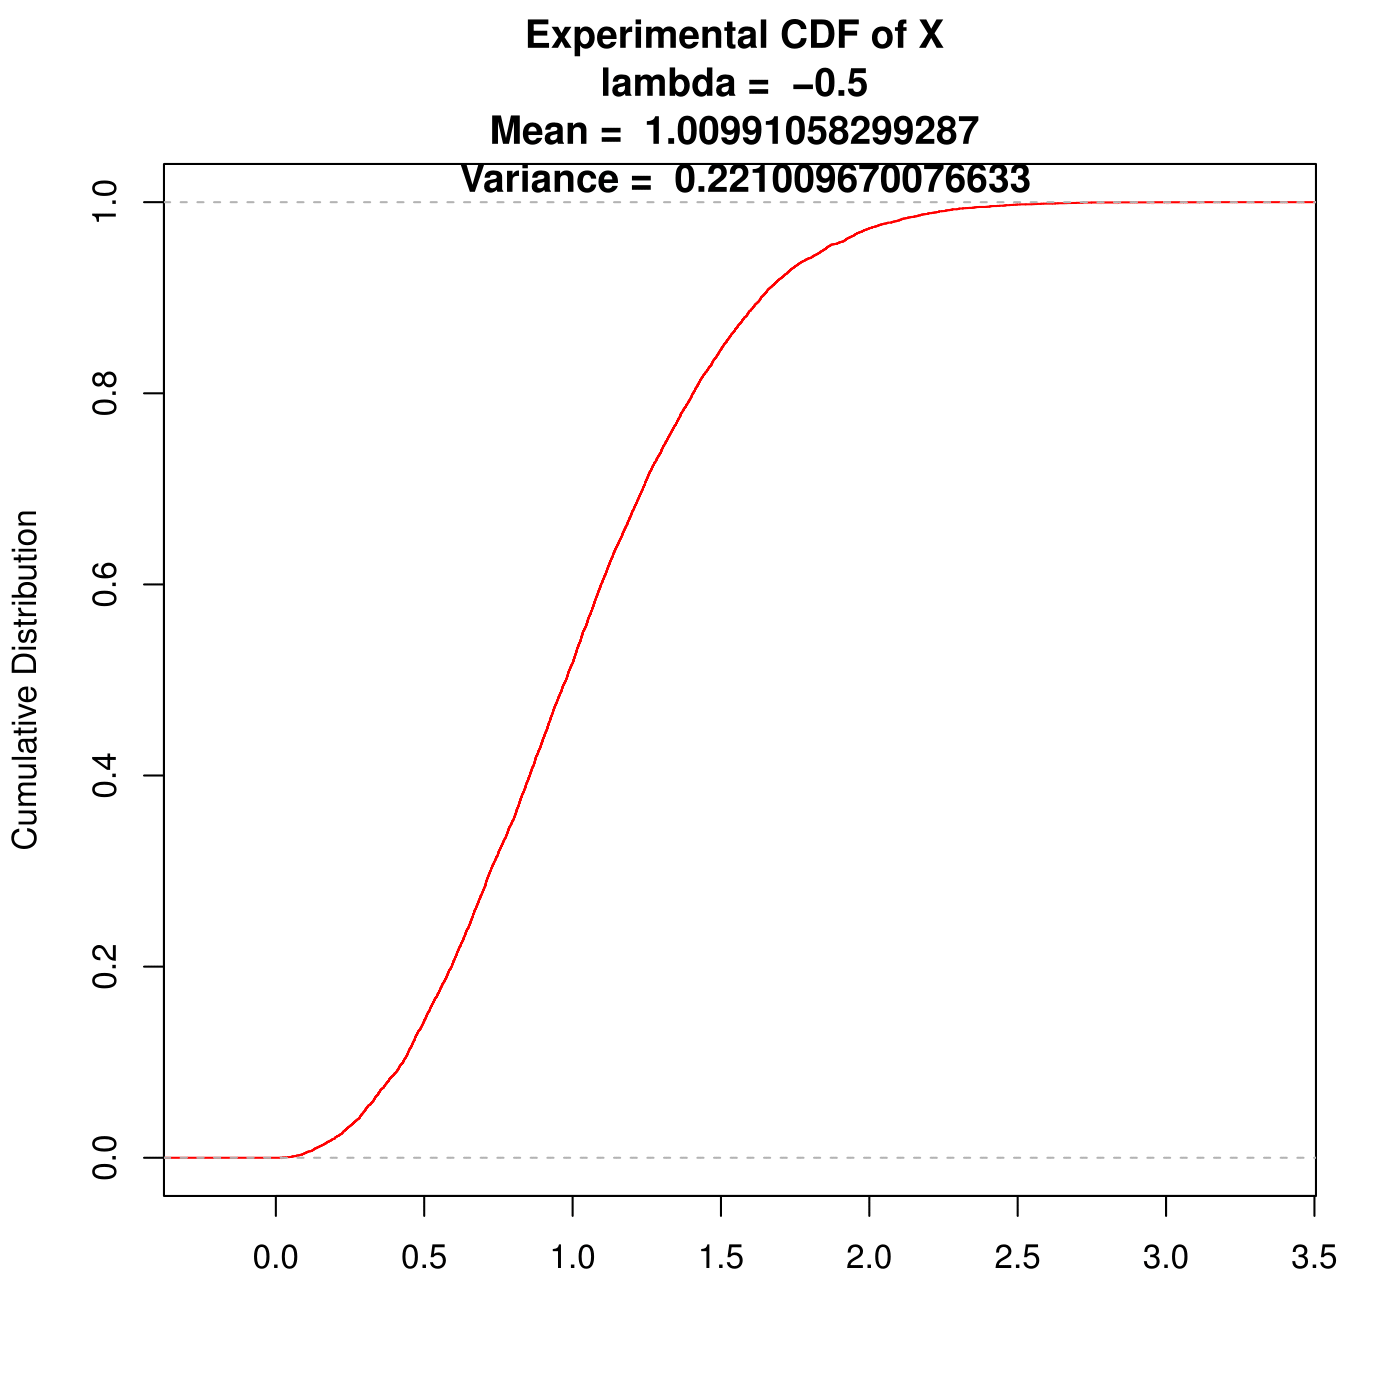
\includegraphics[width=0.90\textwidth]{weibull/Rplots-03.png}{\centering}\\\\
Density of X:\\
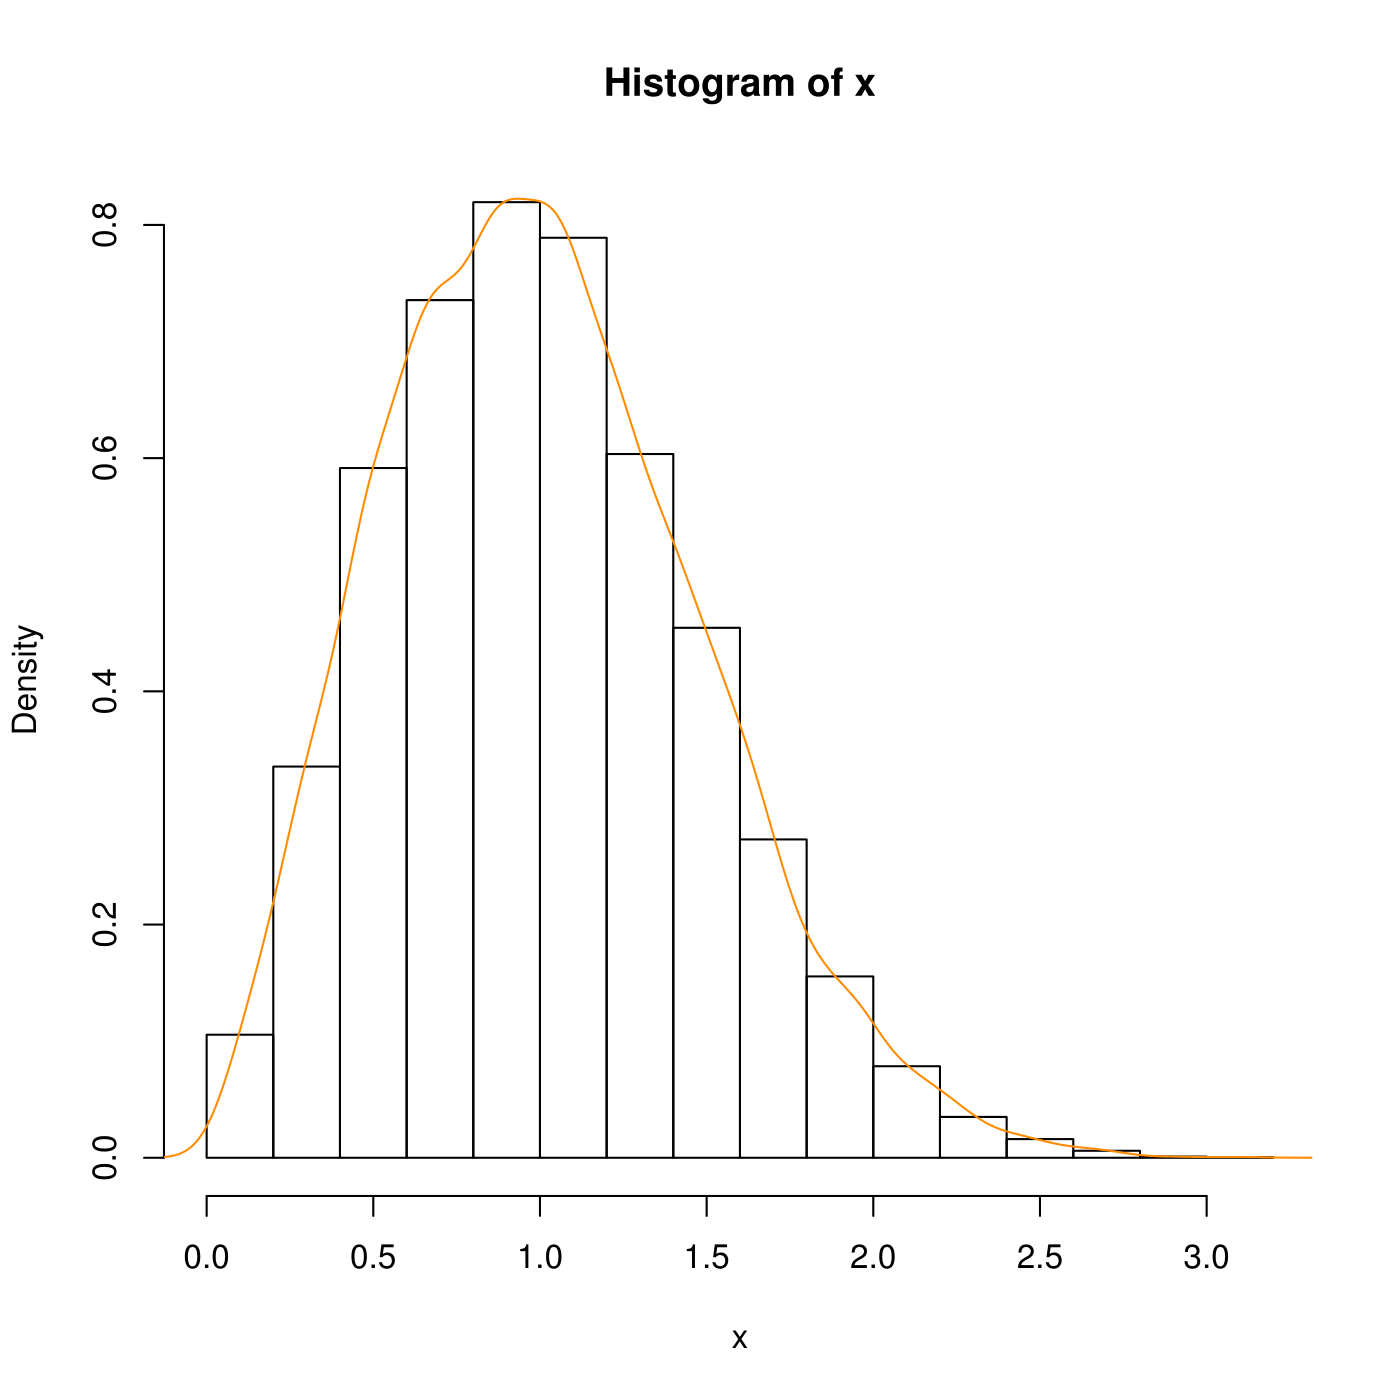
\includegraphics[width=0.90\textwidth]{weibull/Rplots-04.png}{\centering}\\\\
\\For $\lambda=0$\\\\
CDF of X:\\
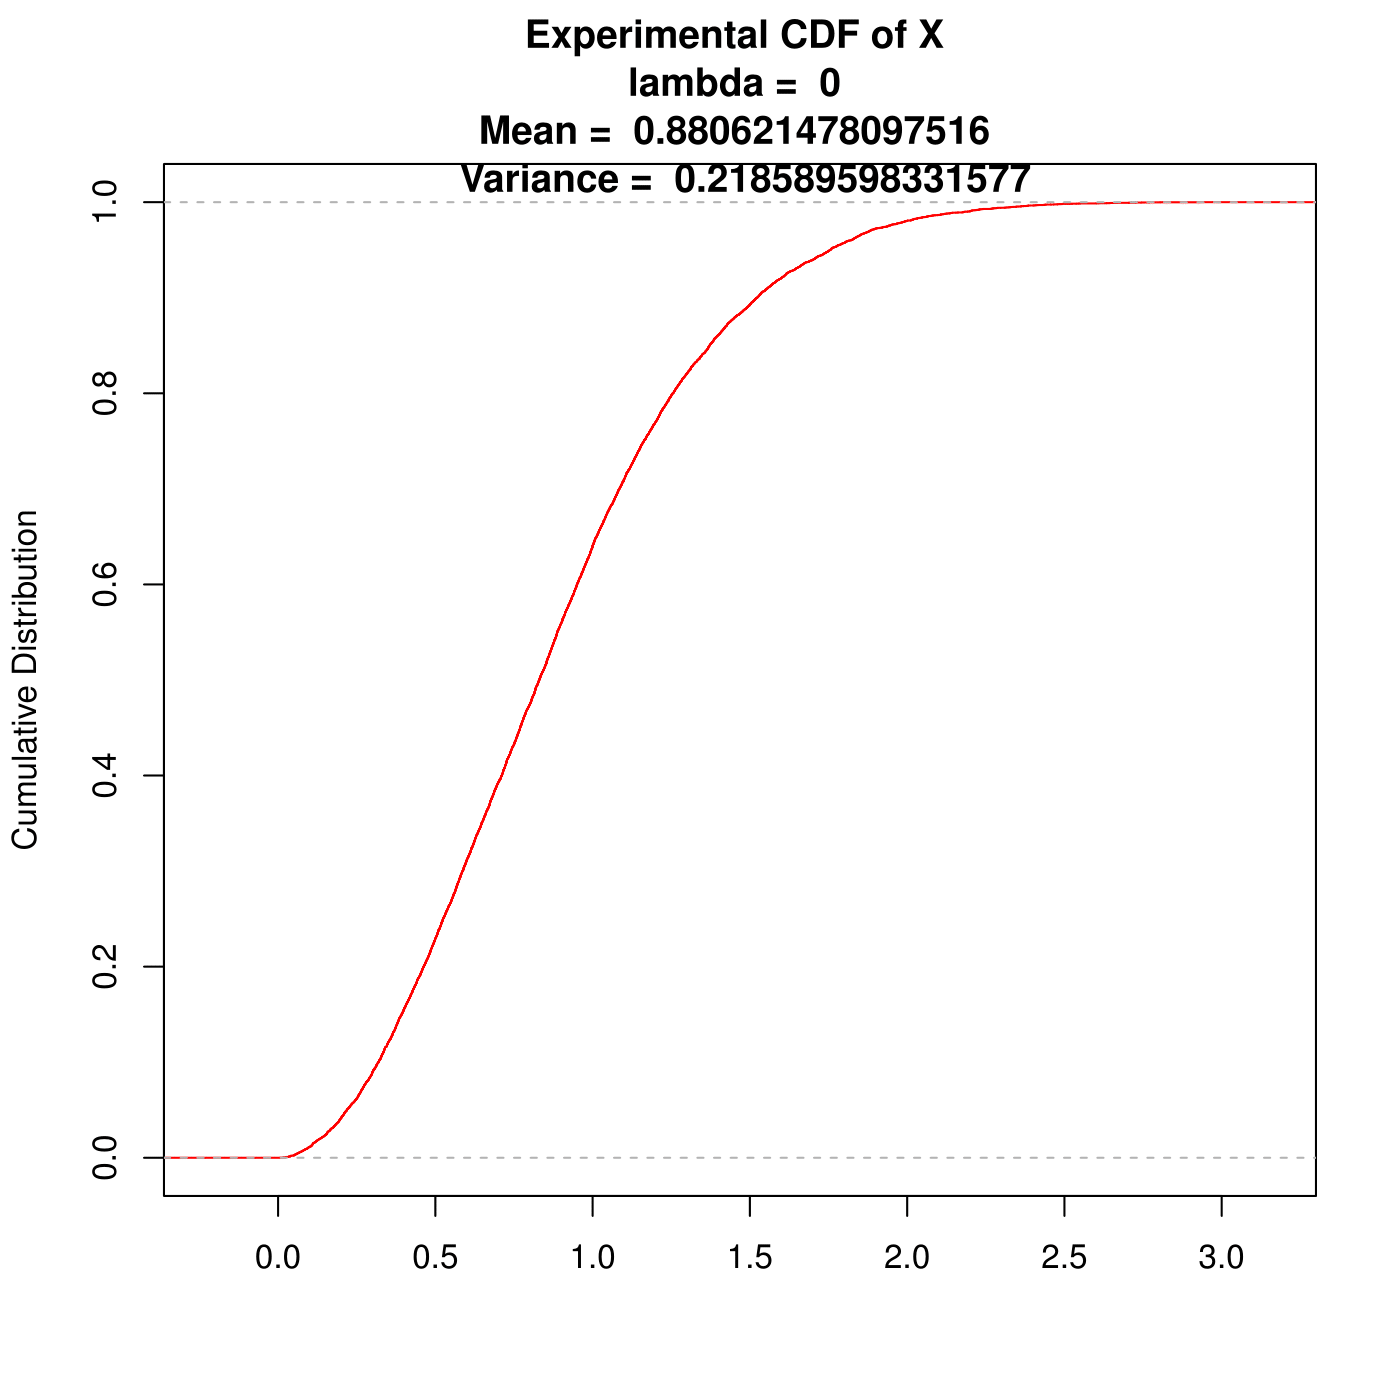
\includegraphics[width=0.90\textwidth]{weibull/Rplots-05.png}{\centering}\\\\
Density of X:\\
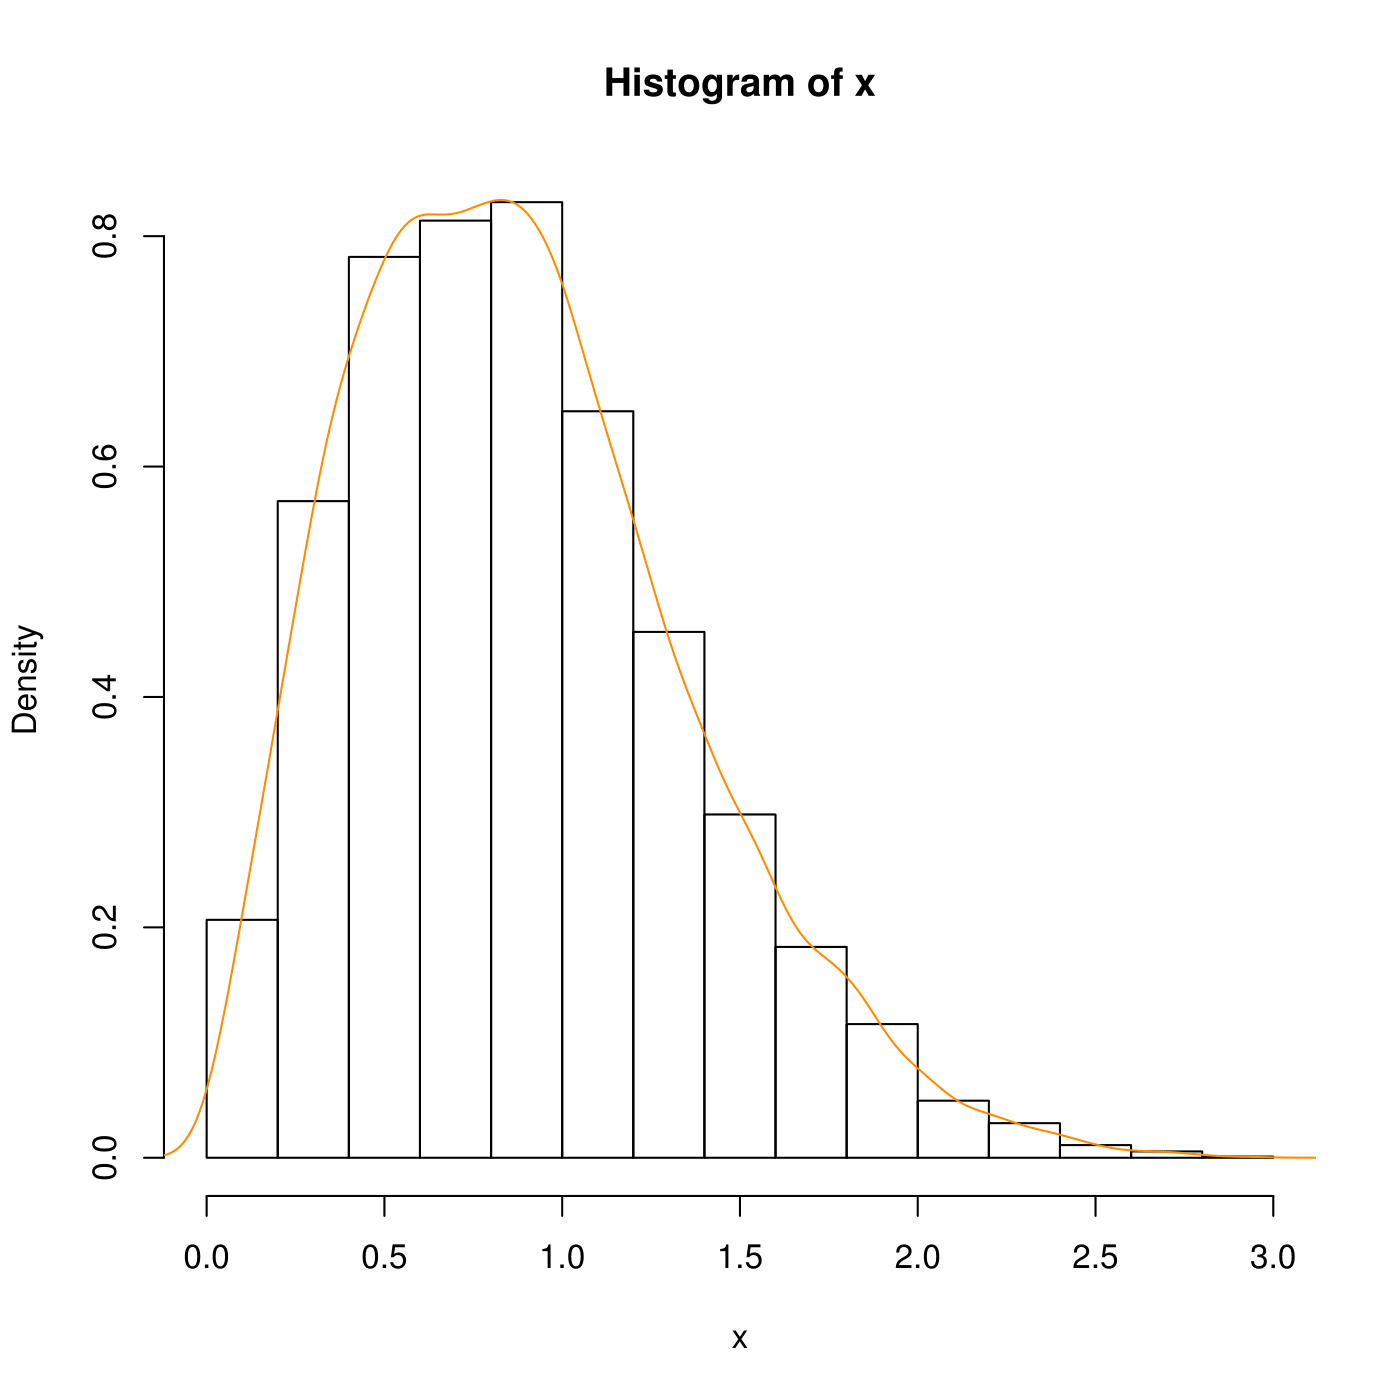
\includegraphics[width=0.90\textwidth]{weibull/Rplots-06.png}{\centering}\\\\
\\For $\lambda=0.5$\\\\
CDF of X:\\
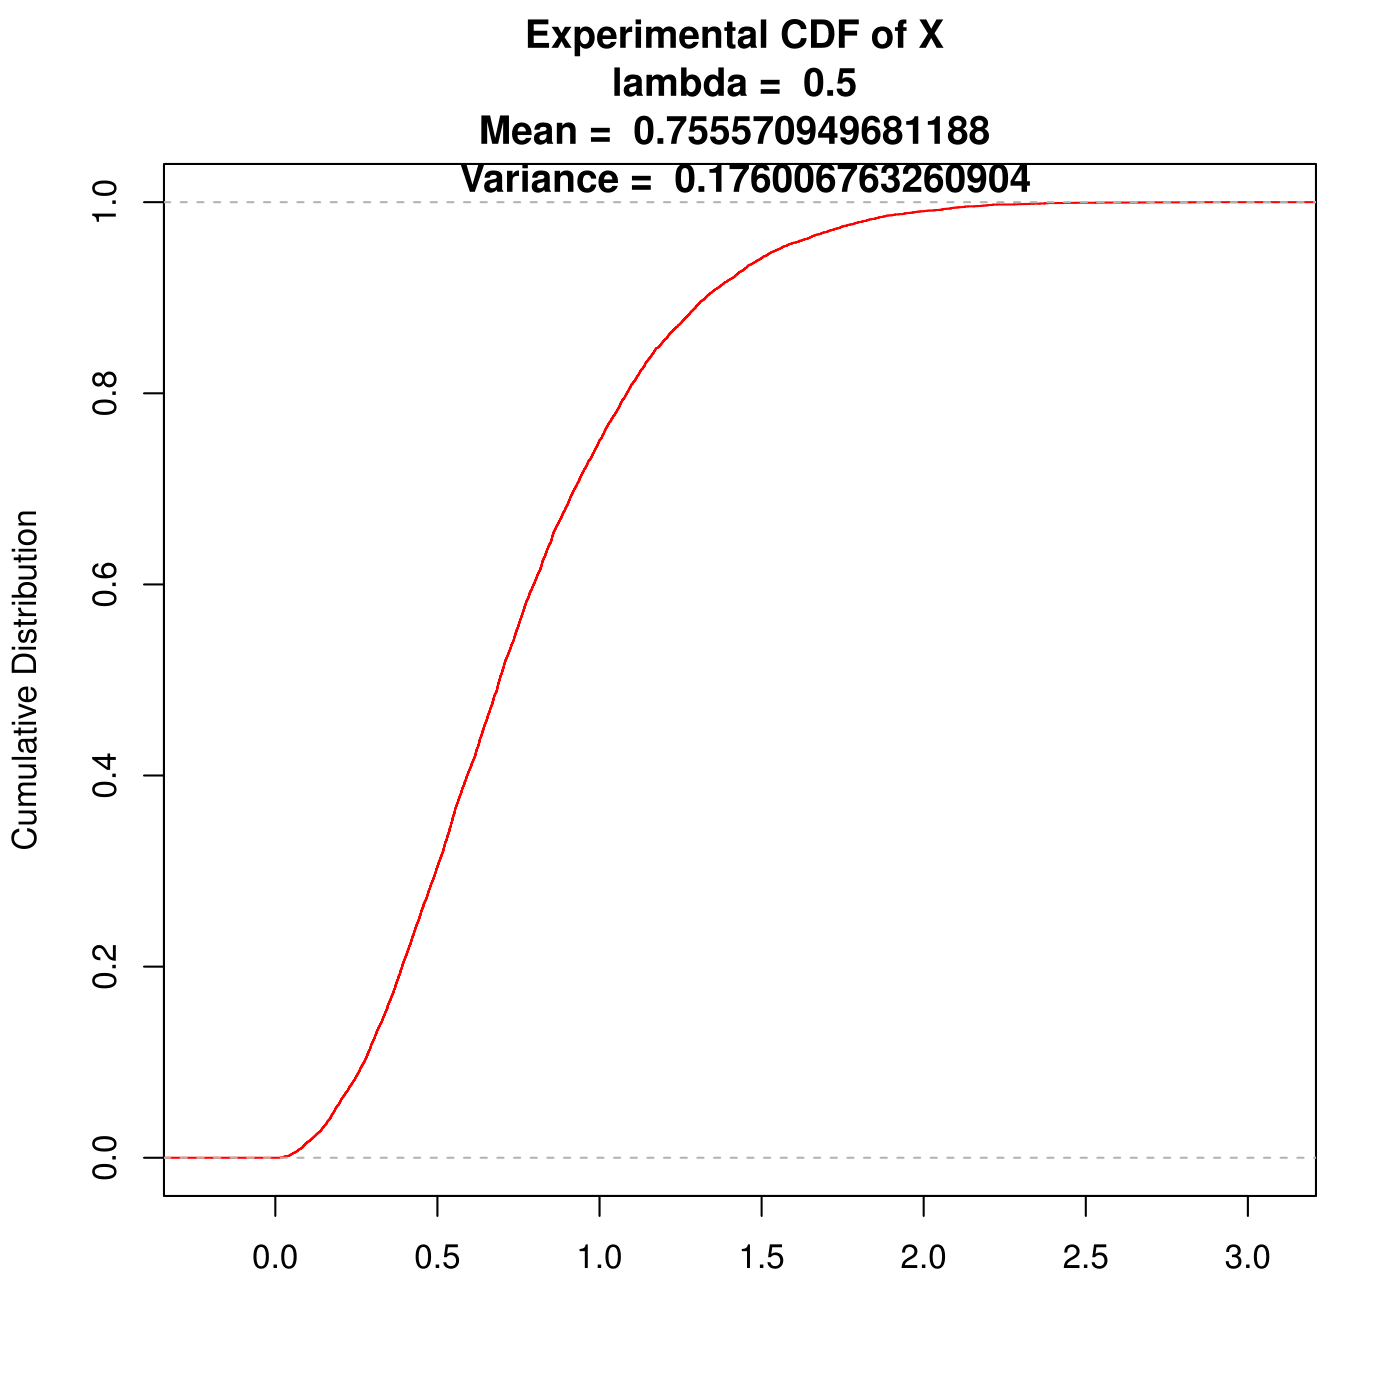
\includegraphics[width=0.90\textwidth]{weibull/Rplots-07.png}{\centering}\\\\
Density of X:\\
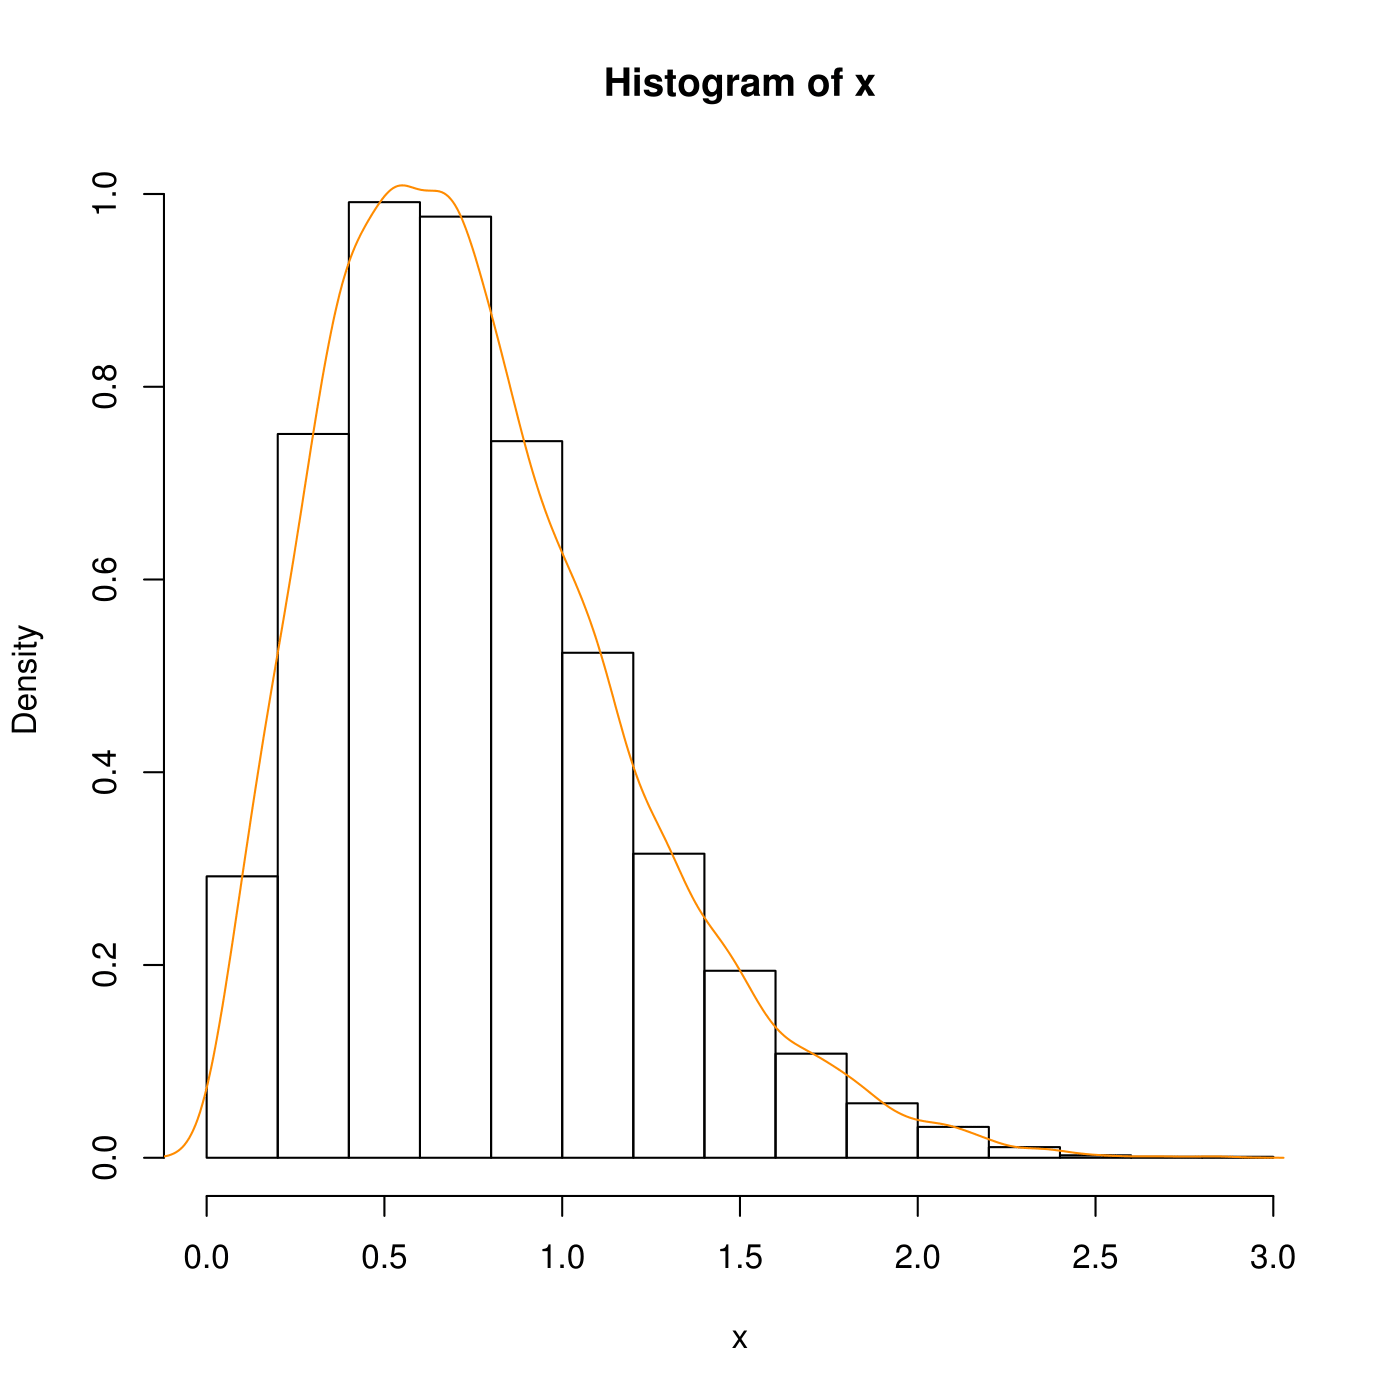
\includegraphics[width=0.90\textwidth]{weibull/Rplots-08.png}{\centering}\\\\
\\For $\lambda=1.0$\\\\
CDF of X:\\
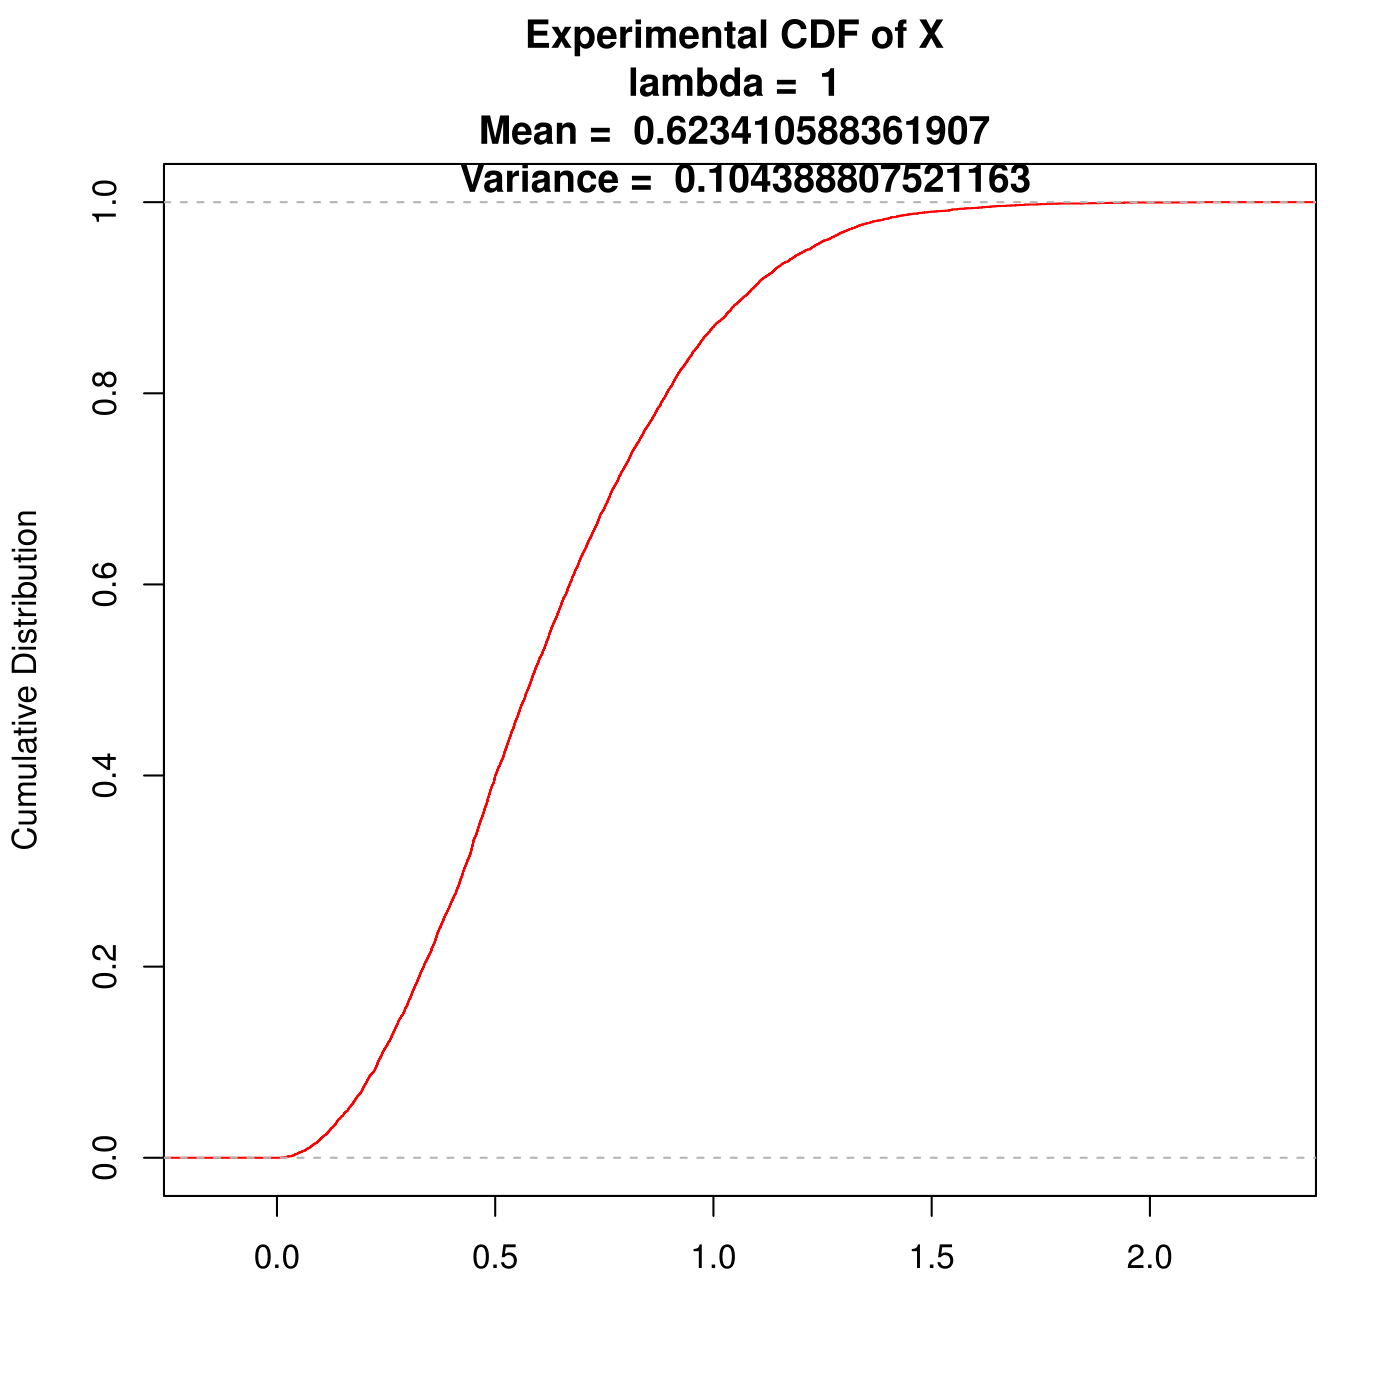
\includegraphics[width=0.90\textwidth]{weibull/Rplots-09.png}{\centering}\\\\
Density of X:\\
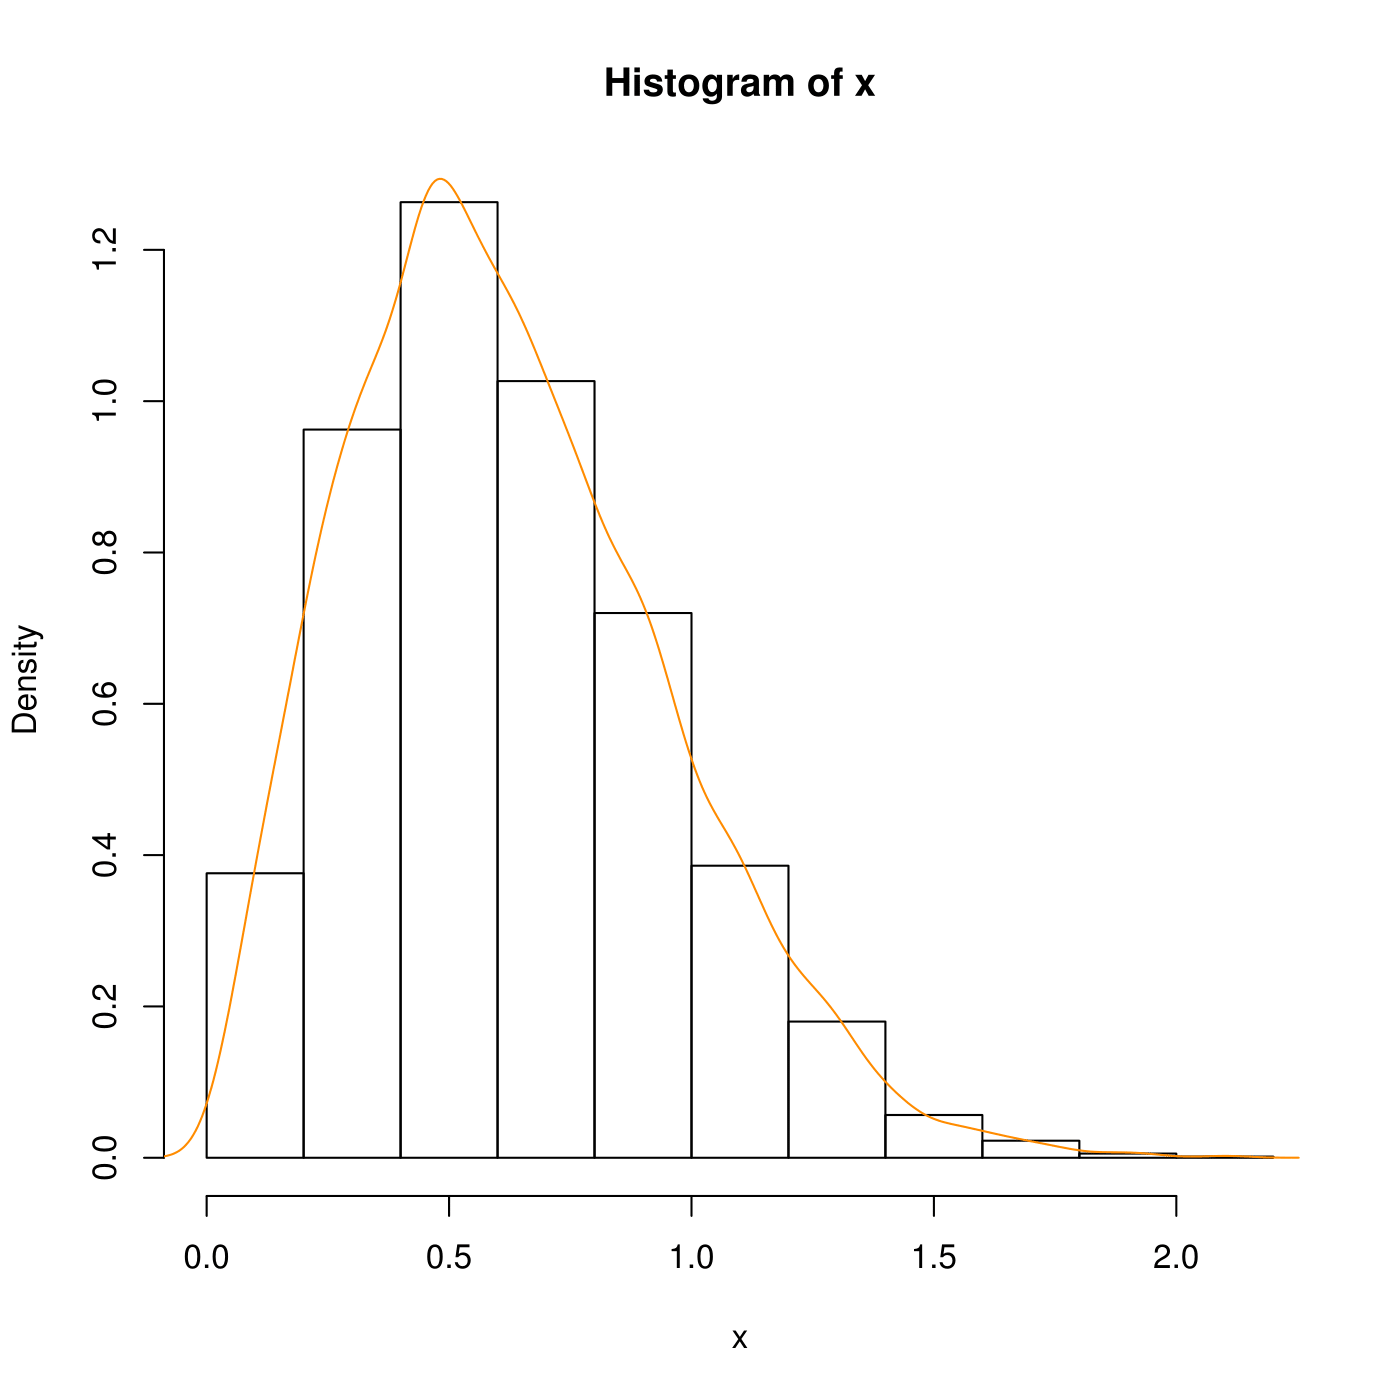
\includegraphics[width=0.90\textwidth]{weibull/Rplots-10.png}{\centering}\\\\
\newpage
\textbf{For Lognormal Distribution:\\}
Probability Density function is\\
$N(lnx;\mu,\sigma)=\frac{1}{\sigma \sqrt{2 \pi}}e^{-\frac{(lnx-\mu)^2}{2 \sigma^2}}$\\
Cumulative density function:\\
$F(x)=\int_{0}^{x}lnN(t;\mu,\sigma)dt=\frac{1}{2}$erfc$[-\frac{lnx-\mu}{\sigma \sqrt{2}}]=\Phi (\frac{lnx-\mu}{\sigma}),x>0$\\
\\erfc=complementary error function \\
$\Phi$=Cumulative distribution function of Normal Distribution.
$F^{*}(x)=(1+\lambda)F-\lambda F^2$\\
$F^{*}(x)=1+(\lambda -1)e^{-\alpha x^{\beta}}-\lambda e^{-2\alpha x^{\beta}}$\\
\\for property 1,\\
Differentiating $F^{*}(x)$\\
$F^{{*}^{'}}(x)=(1+\lambda)\frac {dF}{dx}-2\lambda F\frac {dF}{dx}$\\
$~~~~~~~~~=(1+\lambda-2\lambda F)\frac {dF}{dx}$\\
Since, F is CDF\\
So,$\frac {dF}{dx}>0$ as F is monotonically increasing.\\
Since,$~~0\leq F \leq 1~~$\\
So,$~0\geq-2\lambda F\geq-2\lambda$\\
So,$~1+\lambda\geq(1+\lambda-2\lambda F)\geq1-\lambda$\\
As, $\lambda\geq-1$,\\
So,$F^{{*}^{'}}(x)>0$\\
Hence, it is monotonically increasing function.\\
\\
for property 2\\
$F^{*}(x+) = lim_{n \to\infty}F^{*}(x+\frac1n)=F^{*}(x)$\\
Now , F is CDF. So , F is right continuous.\\
So, $\lambda F^{2}$ is also right continuous.\\
$(1+\lambda)F-\lambda F^{2}$ will also be a right continuous.\\
\textbf{[Sum of continuous function is also a continuous function.]}\\
Hence, $F^{*}$ is right continuous.\\\\
for property 3,\\
$F^{*}(-\infty)=lim_{x \to {-\infty}}F^{*}(x)=0$\\
Since, F is a CDF\\
So, $F(-\infty)=lim_{x \to {-\infty}}F(x)=0$\\
So,$F^{2}(-\infty)=lim_{x \to {-\infty}}F^{2}(x)=0$\\
So,$(1+\lambda)F(-\infty)-\lambda F^{2}(-\infty)=lim_{x \to {-\infty}}((1+\lambda)F(x)-\lambda F^{2}(x))=0$\\
So,$F^{*}(-\infty)=lim_{x \to {-\infty}}F^{*}(x)=0$\\\\
for property 4\\
$F^{*}(\infty)=lim_{x \to {\infty}}F^{*}(x)=1$\\
Since, F is a CDF\\
So, $F(\infty)=lim_{x \to {\infty}}F(x)=1$\\
So,$F^{2}(\infty)=lim_{x \to {\infty}}F^{2}(x)=1$\\
So,$(1+\lambda)F(\infty)-\lambda F^{2}(\infty)=lim_{x \to {\infty}}((1+\lambda)F(x)-\lambda F^{2}(x))=1+\lambda-\lambda=1$\\\\
So,$F^{*}(\infty)=lim_{x \to {\infty}}F^{*}(x)=1$\\\\
Hence $F^{*}$ follows all four properties of Cumulative Distribution function.\\
So, $F^*$ is a  Cumulative Distribution Function.\\
\noindent{Code for R}\\
\begin{lstlisting}
f<-function(b)
{
	u<-runif(1)
	return (((1+b)-sqrt((1+b)^2 - 4*b*u))/(2*b))
}

d<-c(-1,-0.5,0,0.5,1)
x<-1
j<-1
for(j in 1:5)
{
	for(i in 1:10000)
	{
		if(d[j]!=0)
			x[i]<-qlnorm(f(d[j]),meanlog=0,sdlog=1,
		lower.tail=TRUE,log.p=FALSE)
		else
			x[i]<-qlnorm(runif(1),meanlog=0,sdlog=1,
		lower.tail=TRUE,log.p=FALSE)
	}


cat("\nThe Mean of the Distributon calculated is ",mean(x))
cat("\nThe Varinace of the Distributon calculated is ",var(x))
cat("\n")
h=ecdf(x)
plot( h,col="red", xlab="", ylab="Cumulative Distribution",
 main=paste("\nExperimental CDF of X \nlambda = ",d[i],
"\nMean = ",mean(x),"\n Variance = ",var(x))) 
hist(x,ylim=c(0,1),probability='TRUE')
lines(density(x), col='darkorange')

}
\end{lstlisting}
\noindent{Histograms:}\newline
\\For $\lambda=-1$\\\\
CDF of X:\\
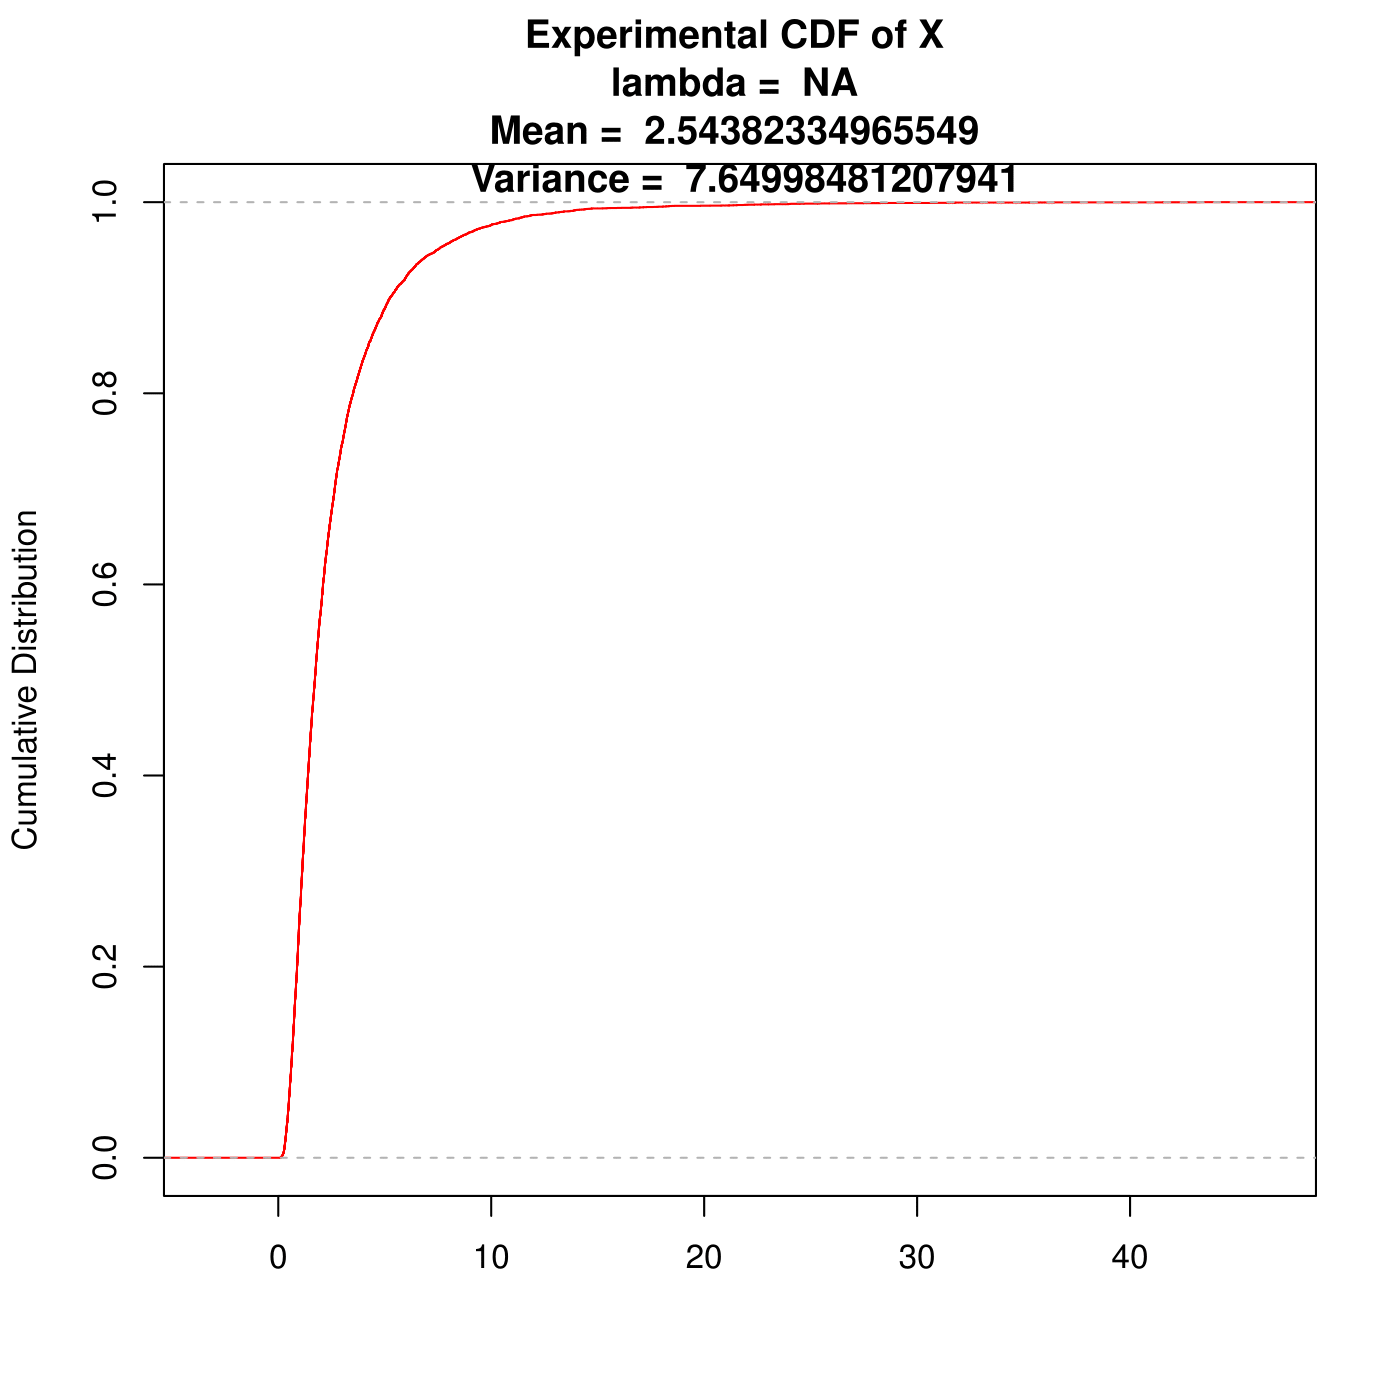
\includegraphics[width=0.90\textwidth]{lnorm/lnorm-01.png}{\centering}\\\\
Density of X:\\
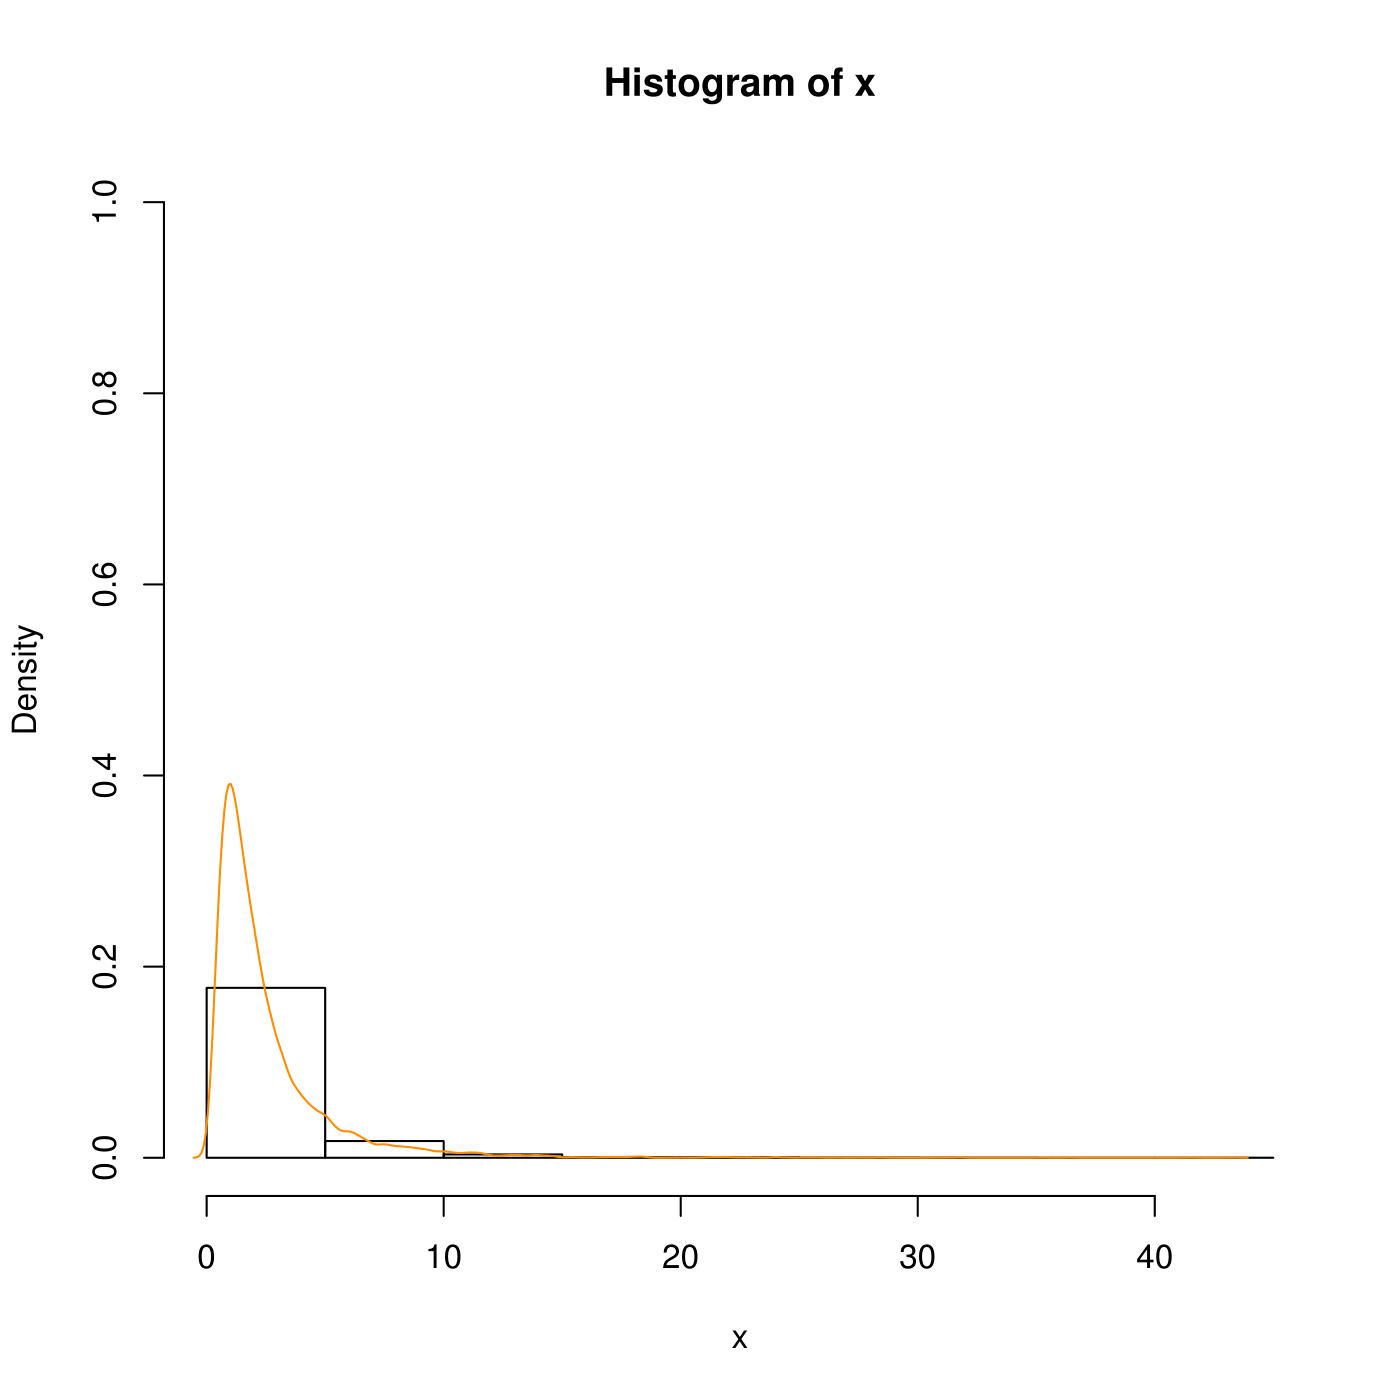
\includegraphics[width=0.90\textwidth]{lnorm/lnorm-02.png}{\centering}\\\\
\\For $\lambda=-0.5$\\\\
CDF of X:\\
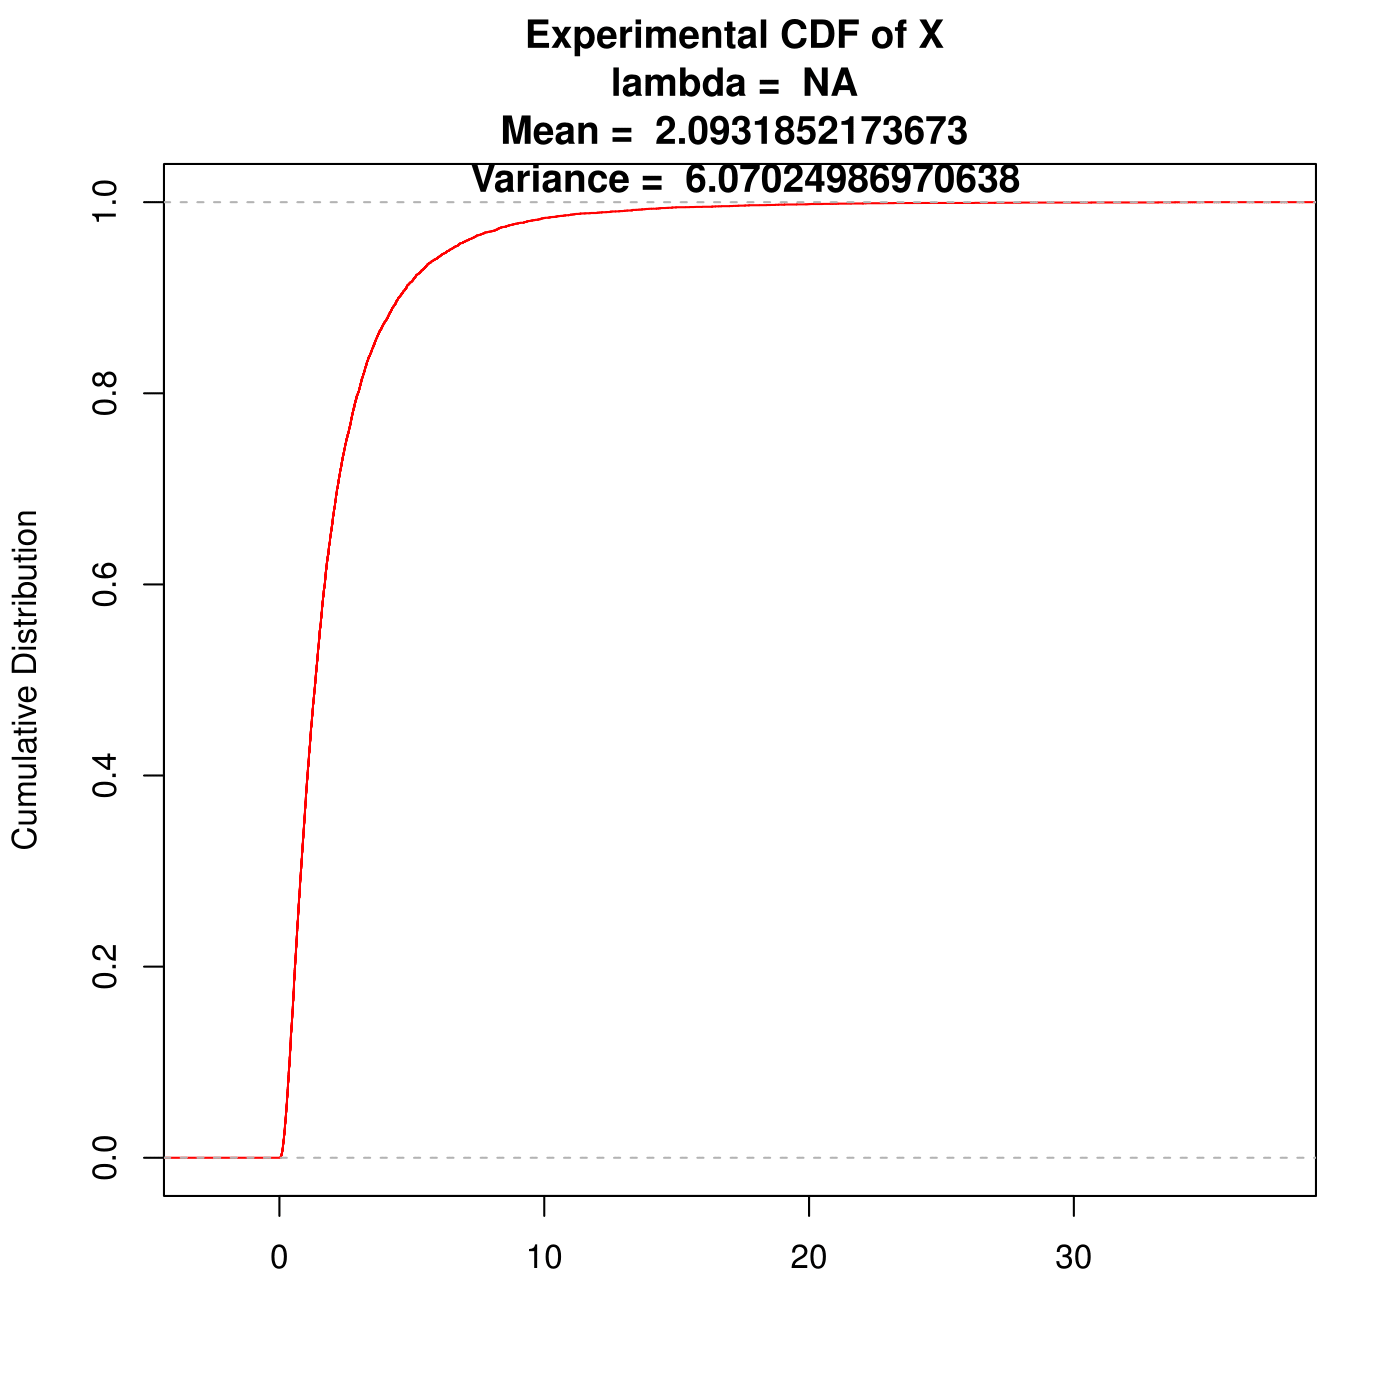
\includegraphics[width=0.90\textwidth]{lnorm/lnorm-03.png}{\centering}\\\\
Density of X:\\
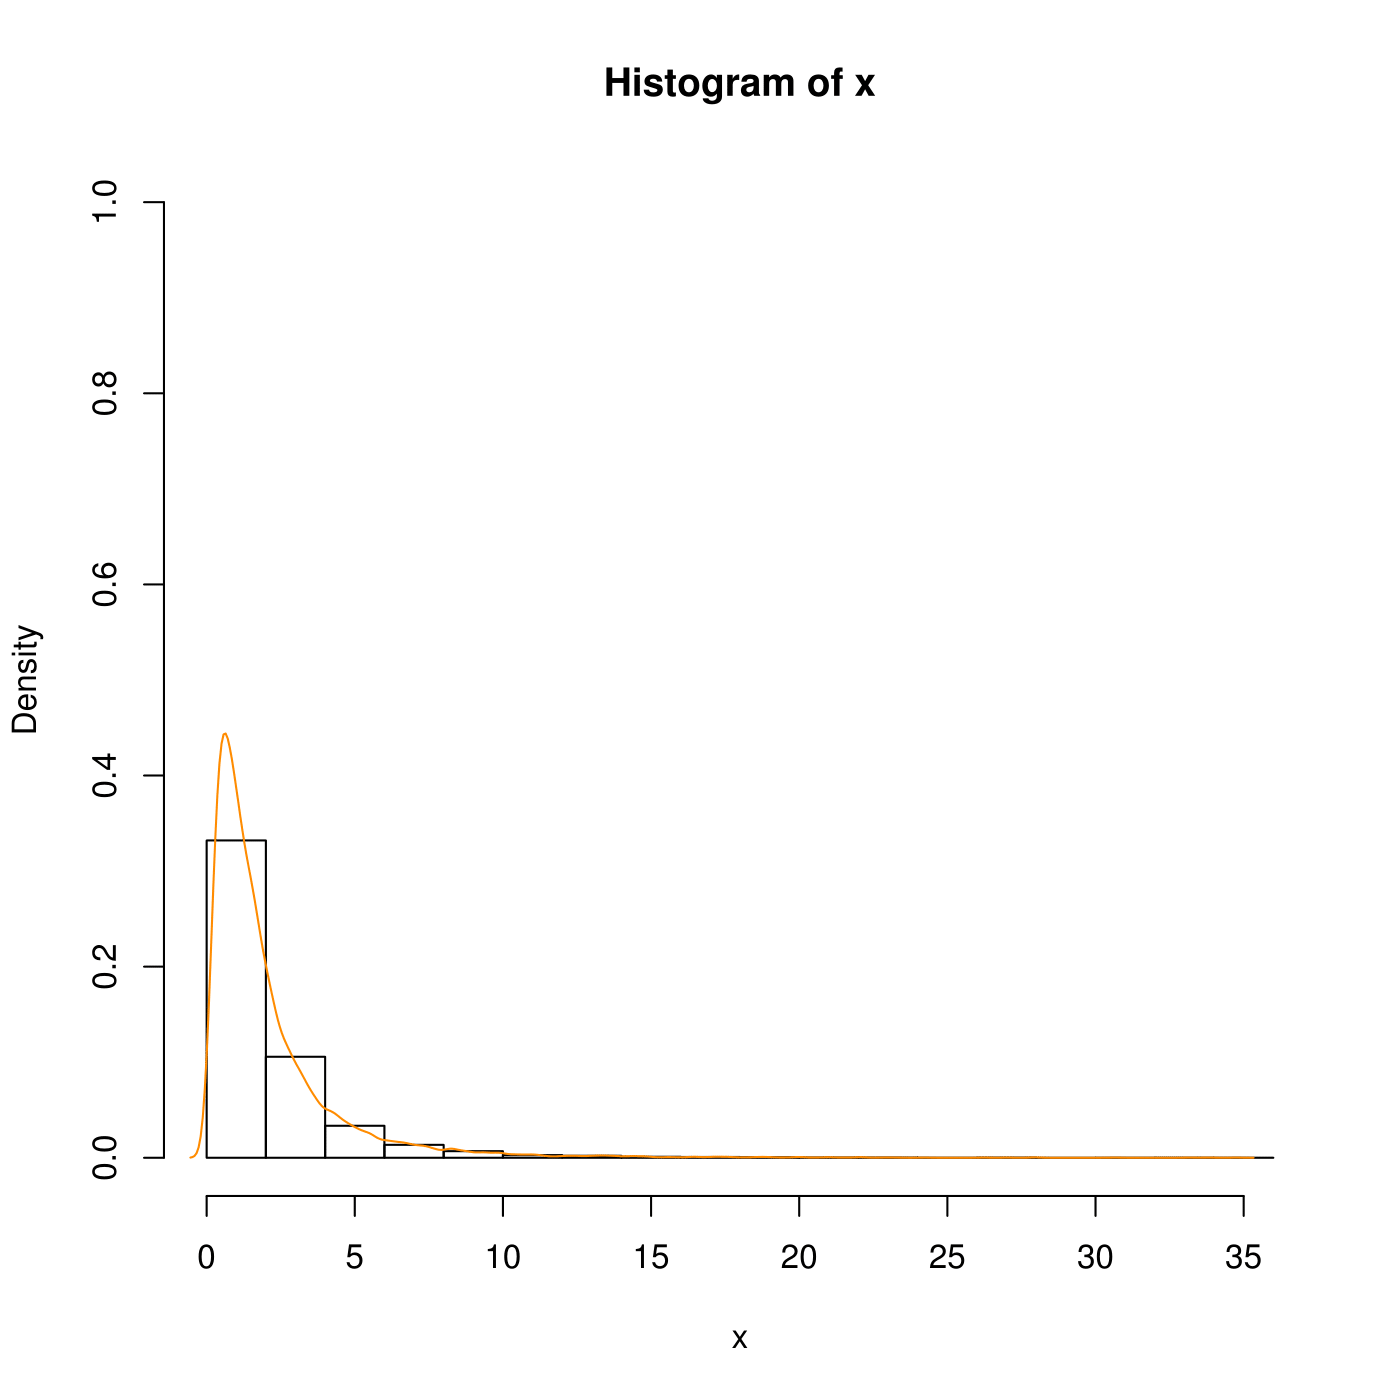
\includegraphics[width=0.90\textwidth]{lnorm/lnorm-04.png}{\centering}\\\\\\
For $\lambda=0$\\\\
CDF of X:\\
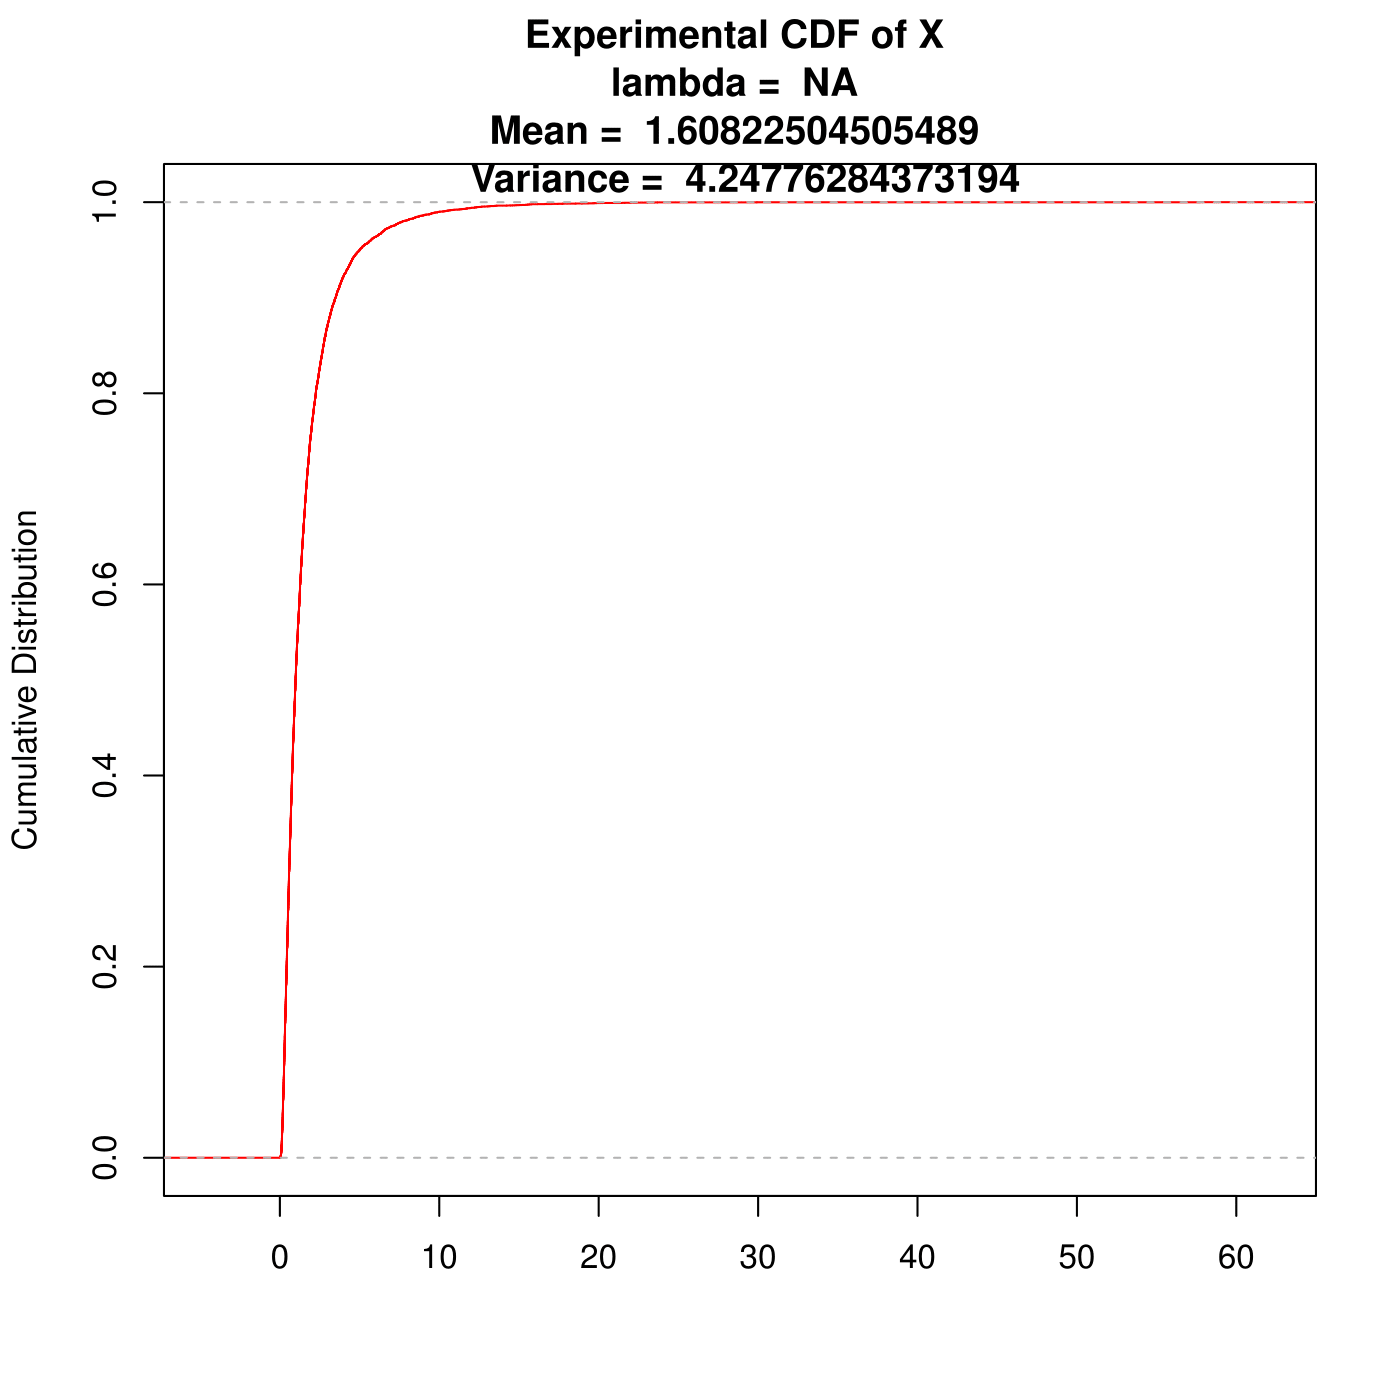
\includegraphics[width=0.90\textwidth]{lnorm/lnorm-05.png}{\centering}\\\\
Density of X:\\
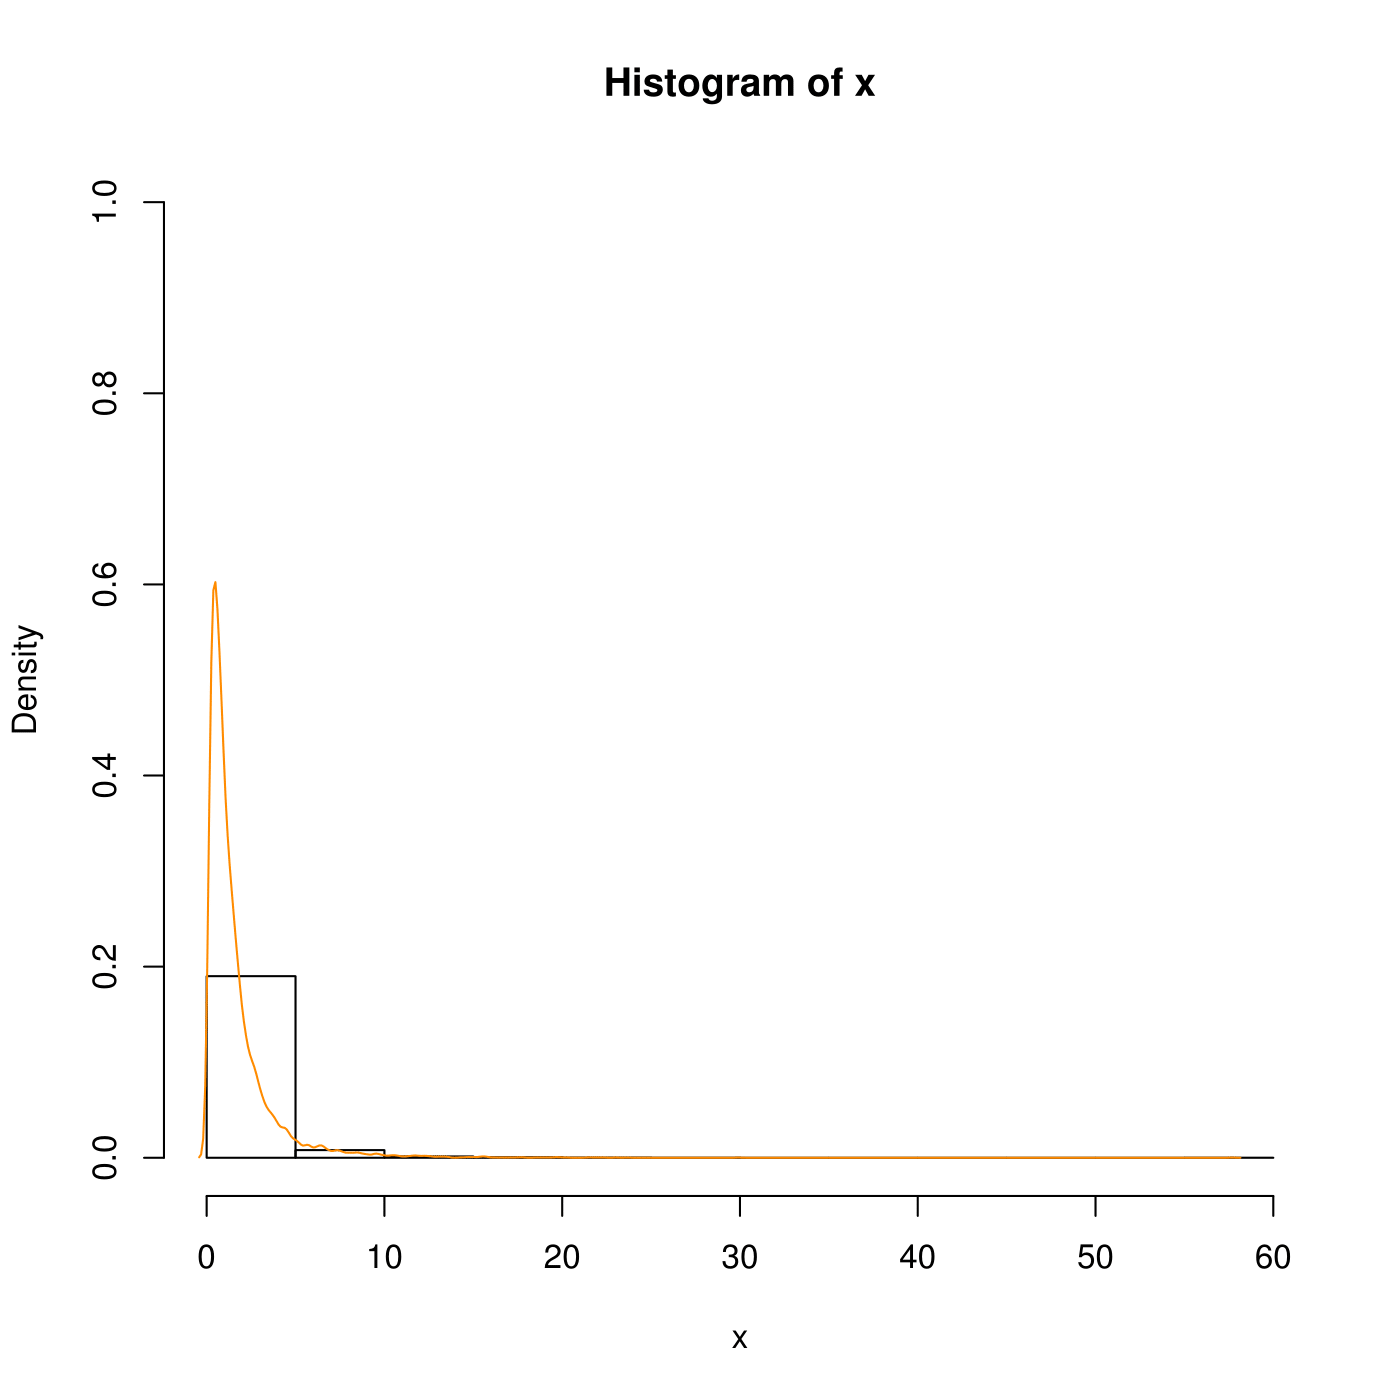
\includegraphics[width=0.90\textwidth]{lnorm/lnorm-06.png}{\centering}\\\\\\
For $\lambda=0.5$\\\\
CDF of X:\\
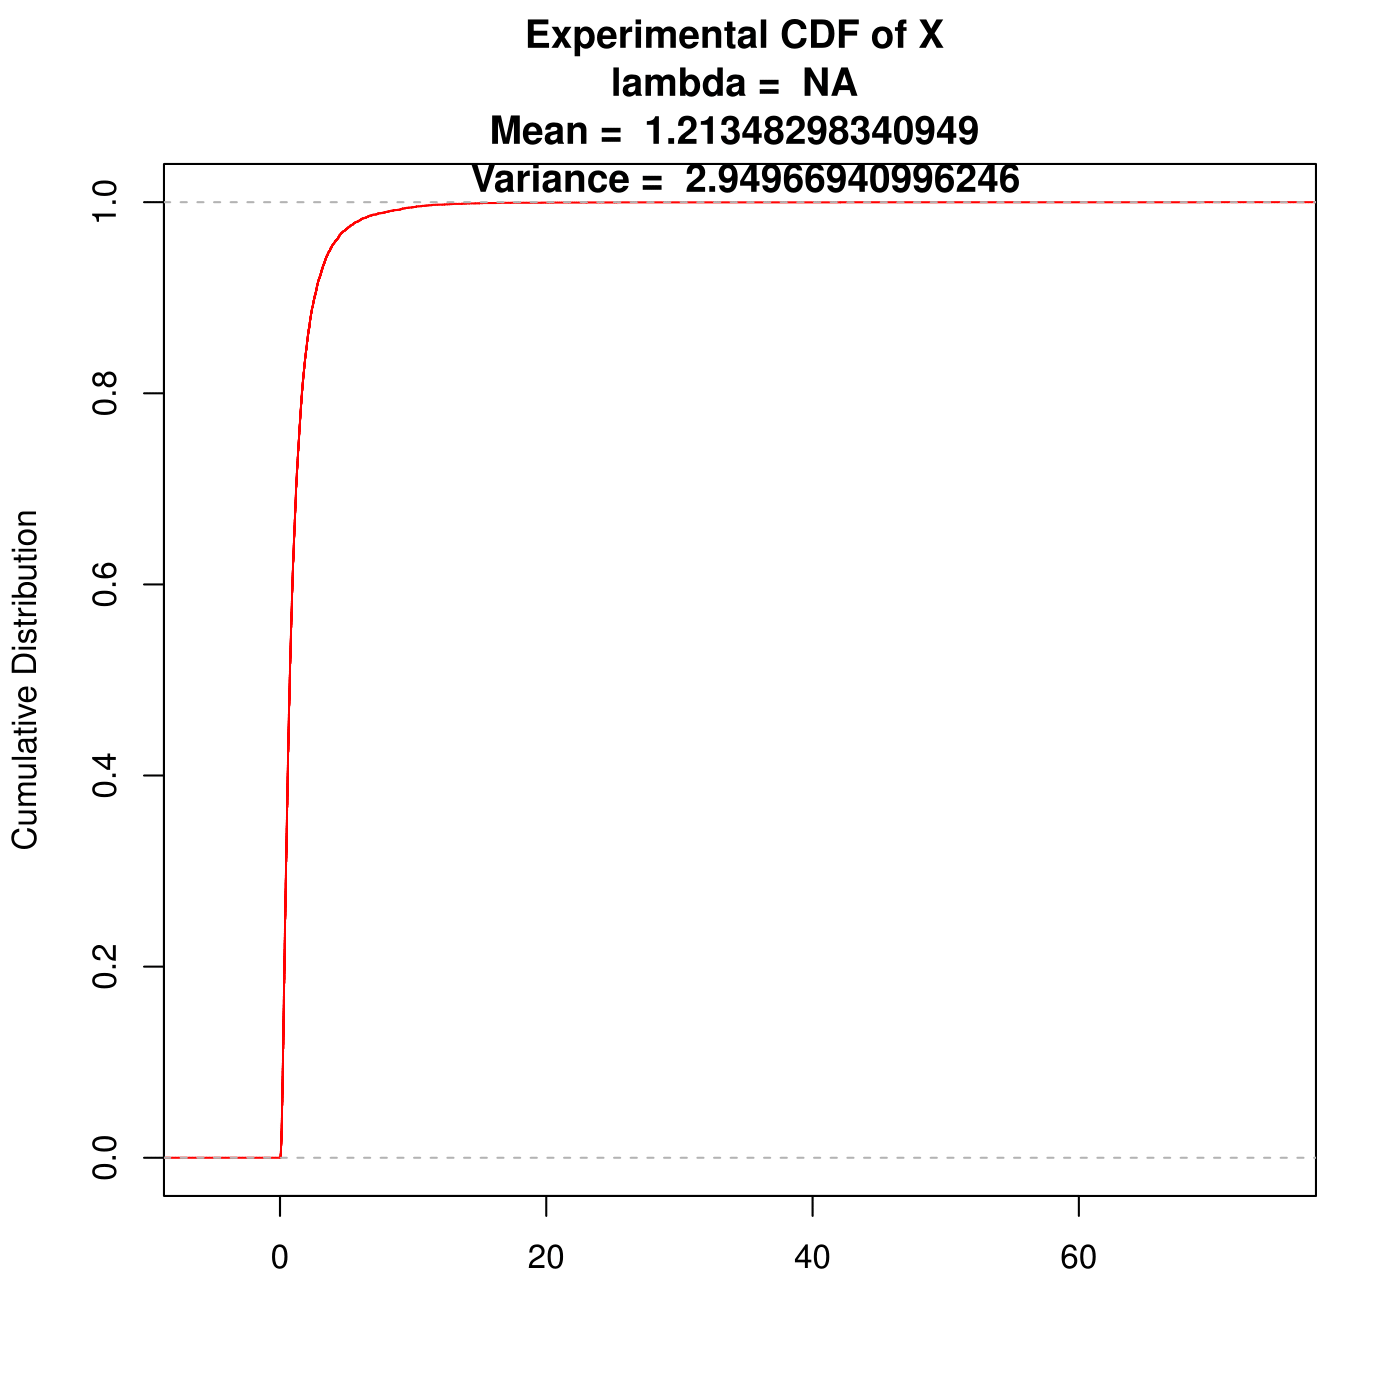
\includegraphics[width=0.90\textwidth]{lnorm/lnorm-07.png}{\centering}\\\\
Density of X:\\
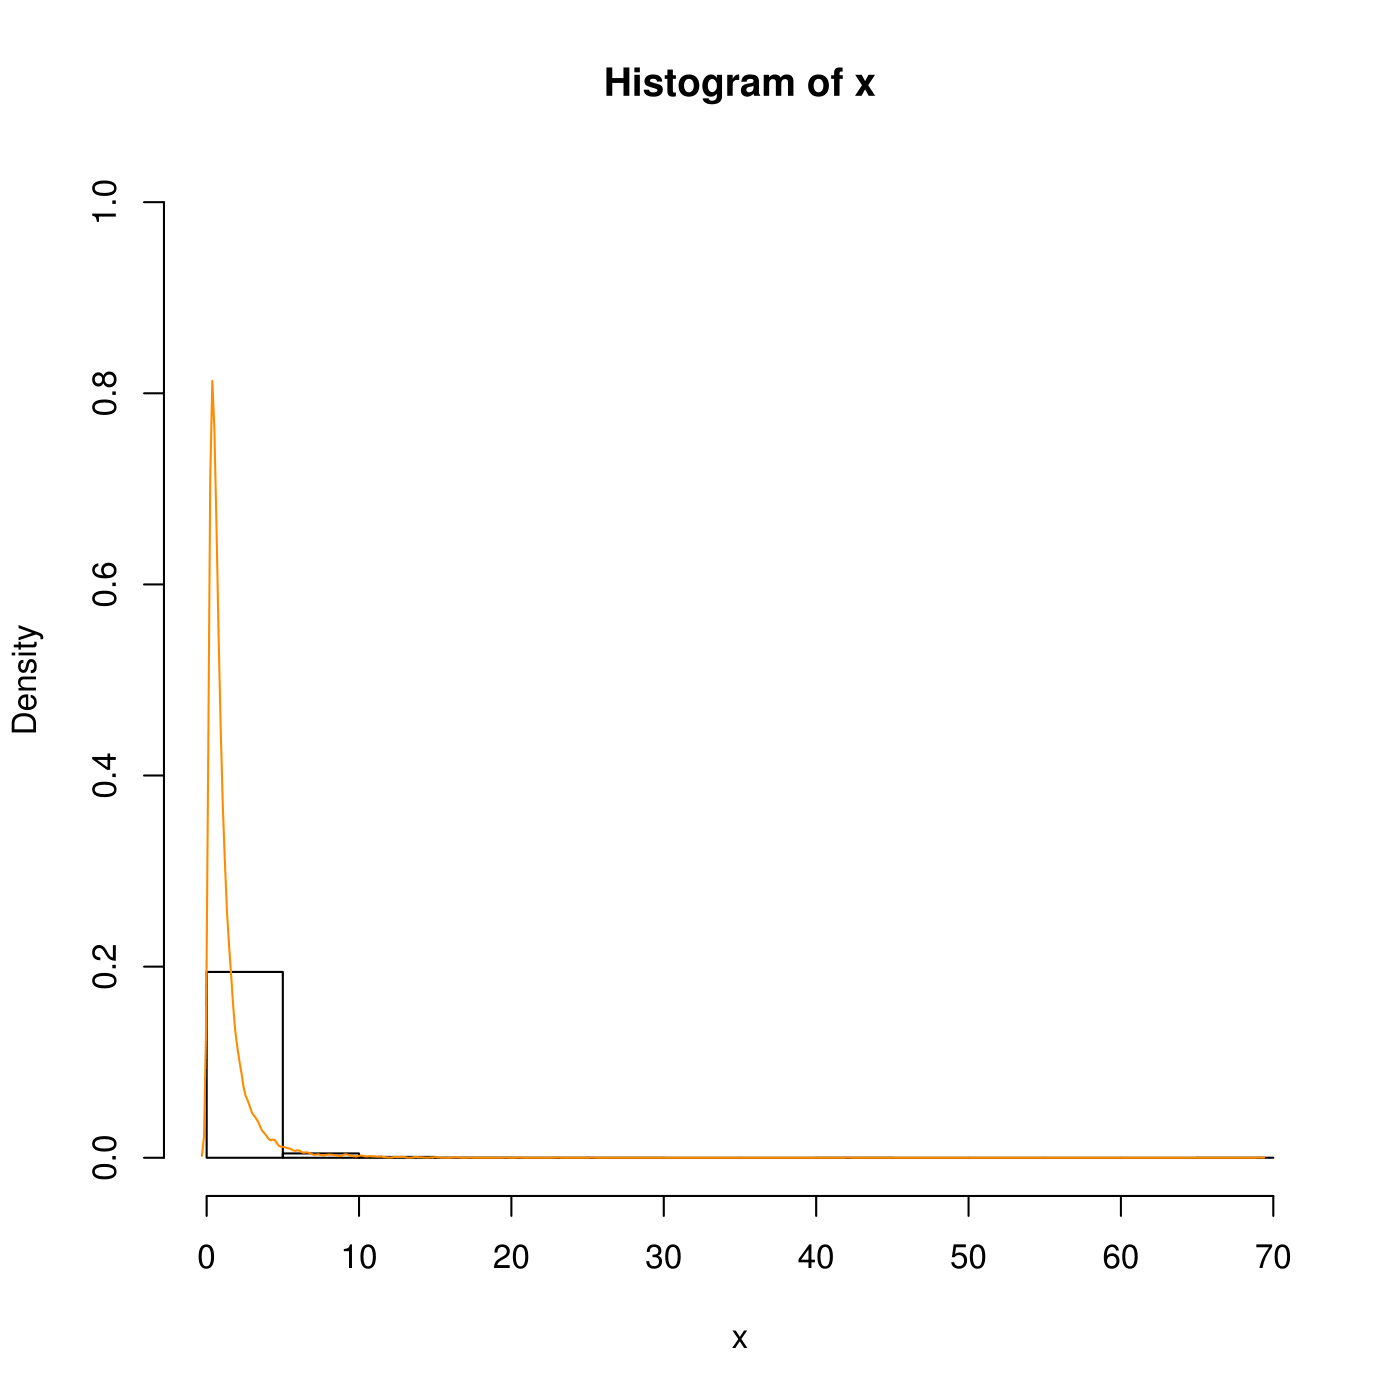
\includegraphics[width=0.90\textwidth]{lnorm/lnorm-08.png}{\centering}\\\\\\
For $\lambda=1$\\\\
CDF of X:\\
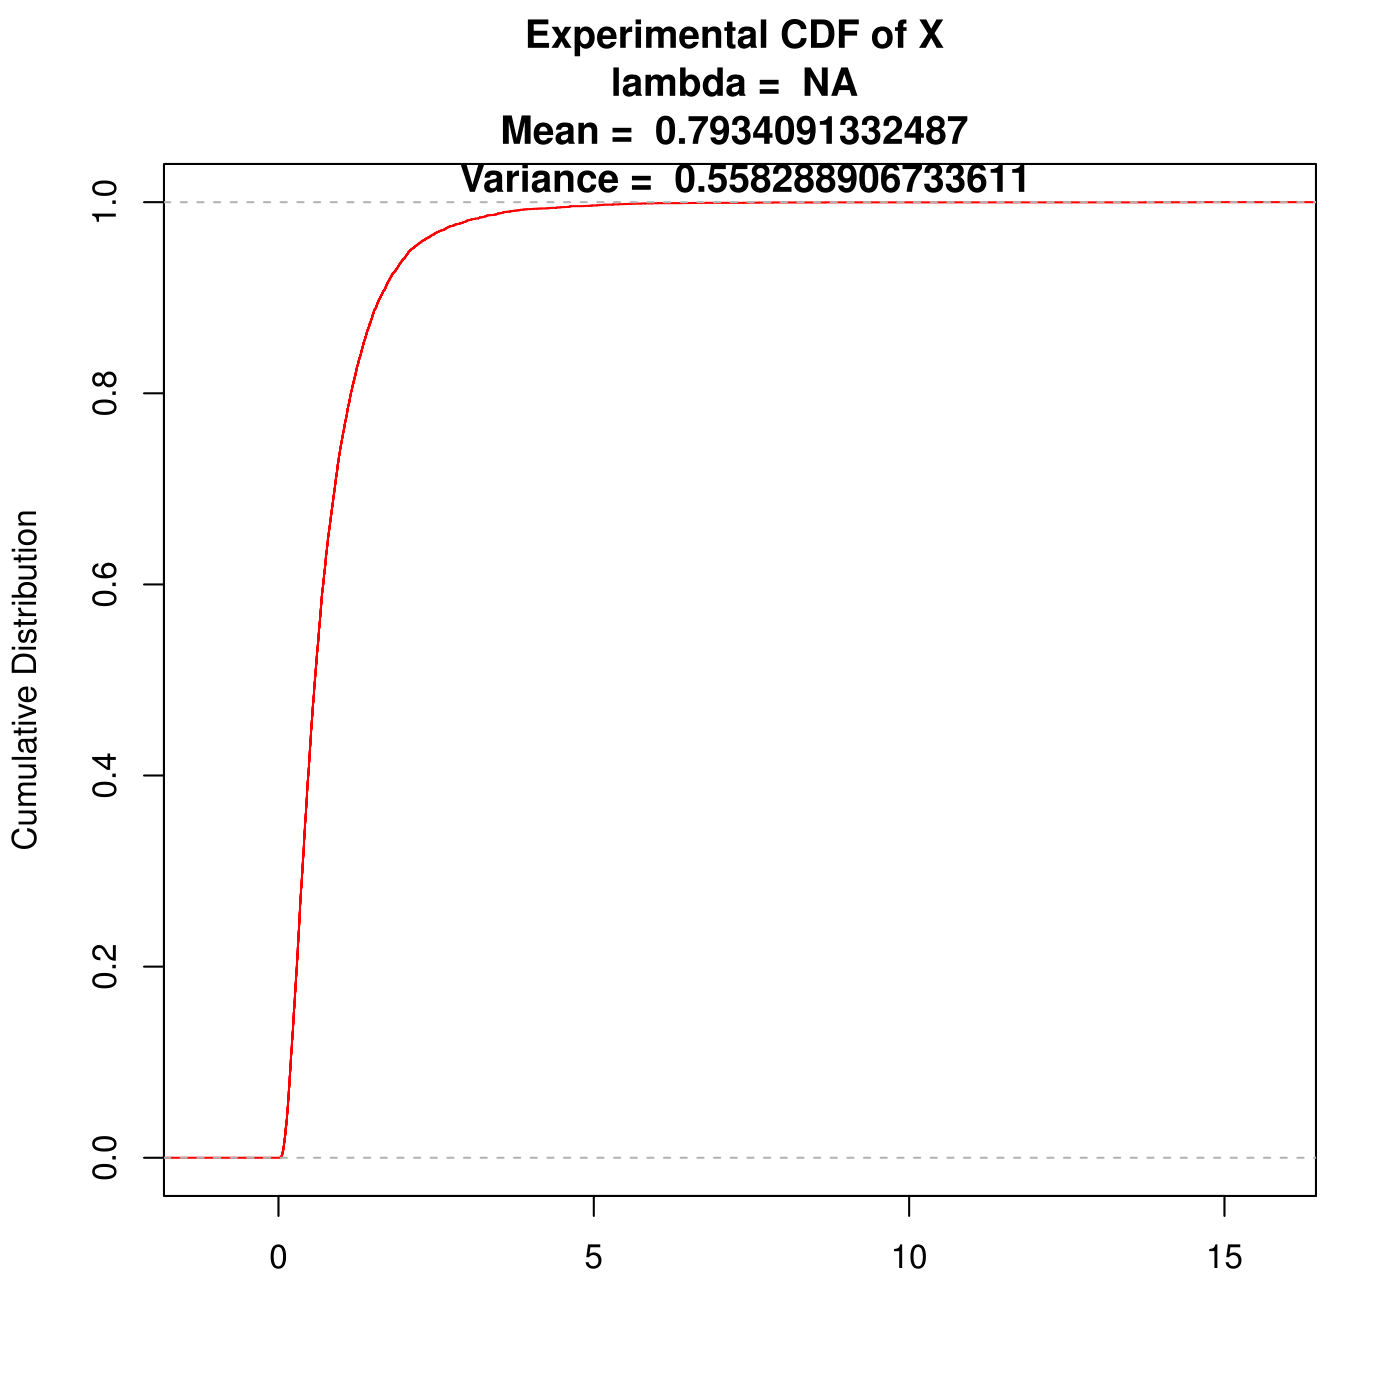
\includegraphics[width=0.90\textwidth]{lnorm/lnorm-09.png}{\centering}\\\\
Density of X:\\
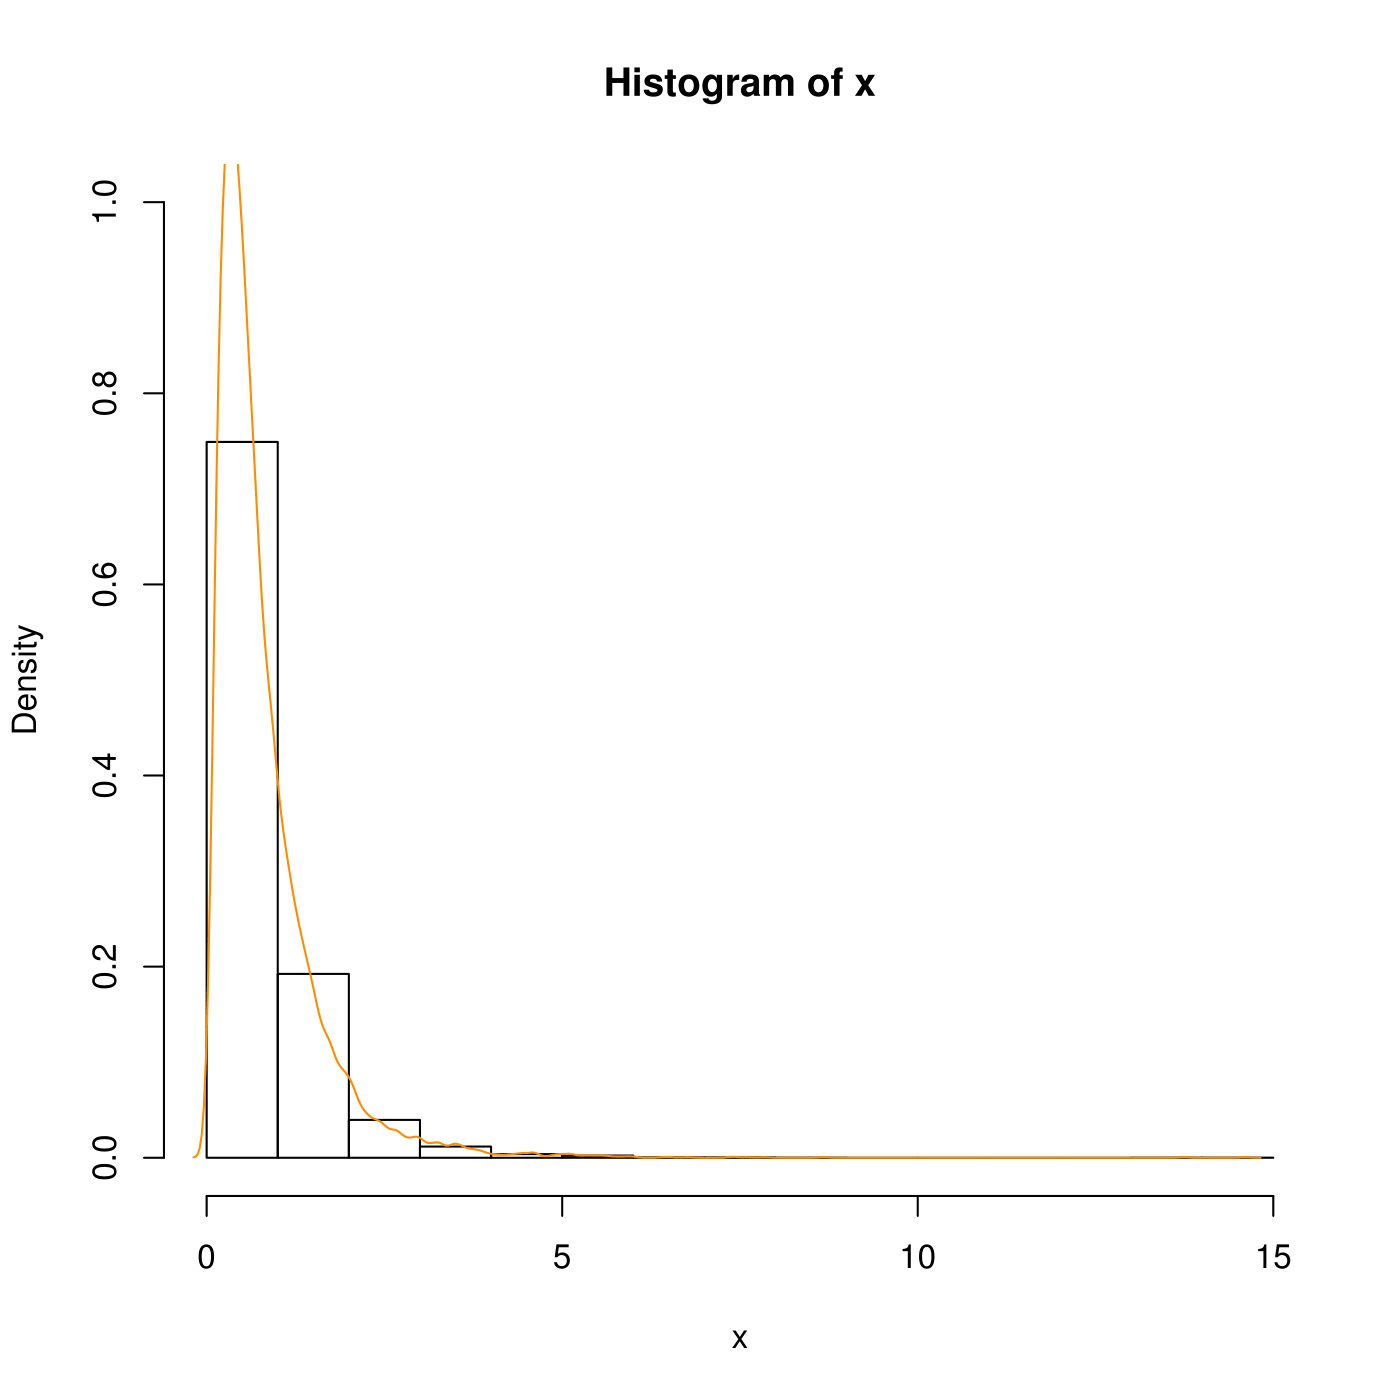
\includegraphics[width=0.90\textwidth]{lnorm/lnorm-10.png}{\centering}\\\\\\
\newpage
\begin{enumerate}
\item[\textbf{Q2:}]
\textbf{ Use Marshall Olkin Weibull Distribution to generate random numbers having  the CDF $F^{*}$ such that $\lambda$ satisfies $-1\leq\lambda\leq1$,\\
$F^{*}(x)=(1+\lambda)F-\lambda F^2$ ,\\
}

\item[Ans:]

\end{enumerate}
\textbf{We have Marshall Olkin Weibull Distribution which is given as follows :}\\\\
$W_{1}=1-e^{- \alpha_{}x^{\beta_{1}}}$\\
$W_{2}=1-e^{- \alpha_{}x^{\beta_{2}}}$\\
$W_{3}=1-e^{- \alpha_{}x^{\beta_{3}}}$\\
These are 3 webull distributions.\\
Marshall Olkin Weibull Distribution is bivariate in nature given by two random variables :\\
$X_{1}=min(w_{1},w_{2})$\\
$X_{2}=min(w_{1},w_{3})$\\
$(X_{1},X_{2})$ follows this distribution.\\
Now , F is its CDF which depends on $\alpha_{},\beta_{1},\beta_{2},\beta_{3}$.Also , its probability density function depends on these parameters.\\
So, now $F^{*}(X)=(1+\lambda)F-\lambda F^2$\\
$f^{*}(x) $ is the pdf of the new distribution.\\
Upon differentiating $F^{*}(x)$ we get :\\
$f^{*}(x) ~= (1+\lambda)f - 2\lambda(Ff + f_{x}f_{y})$\\
Moreover in Marshall Olkin Weibull Distribution:\\
$Ff=f_{x}f_{y}$\\
So,$f^{*}(x) ~= (1+\lambda)f - 2\lambda(2Ff)$\\
Hence,$f^{*}(x) ~= (1+\lambda)f - 4\lambda(Ff)$..............\textbf{1)}\\\\

By acceptance rejection method:
$f(x)=\frac{d^{2}F(x_{1},x_{2})}{dx_{1}dx_{2}}$\\
So,$\frac{f^{*}(x)}{f(x)}\leq c $ where c $\in \mathbb{R}$\\
Now, from 1) \\
$\frac{f^{*}(x)}{f(x)} =\frac{(1+\lambda)f-4\lambda fF}{f}  $.......\textbf{2)}\\\\
So,maximum value  is attained when F=1\\
Hence,putting F=1 in 2) we get,\\
$c \geq (1-3\lambda)$\\
So, we get the value of c as atleast 1-3$\lambda$.
\\\\\\\\
\noindent{Code for R}\\
\begin{lstlisting}
library(MASS)
#F* = (1+lamda)F - (lamda)^2

# 1-D Weibull
weibull_pdf_1d <- function(x, alpha, theta)
{
	return (alpha * theta * x^(alpha - 1) * exp(-theta * x^alpha))
}

weibull_se_1d <- function(x, alpha, theta)
{
	return (exp(-theta * x^alpha))
}

weibull_cdf_1d <- function(x, alpha, theta)
{
	return (1 - weibull_se_1d(x, alpha, theta))
}

#Generates n 1-D weibull numbers with given parameters
weibull_generator_1d <- function(alpha, theta, n)
{
	u <- runif(n)
	return (((-1/theta) * log(u))^(1/alpha))
}

# 2-D Marshall-Olkin bivariate Weibull
mobw_pdf_2d <- function(x1, x2, alpha, lamda0, lamda1, lamda2)
{
	if(x1 < x2)
	{
		return (weibull_pdf_1d(x1, alpha, lamda1) *
		 weibull_pdf_1d(x2, alpha, lamda0 + lamda2))
	}
	else if (x1 > x2)
	{
		return (weibull_pdf_1d(x1, alpha, lamda0 + lamda1) *
		 weibull_pdf_1d(x2, alpha, lamda2))
	}
	else
	{
		return ((lamda0/(lamda0 + lamda1 + lamda2)) *
		 weibull_pdf_1d(x1, alpha, lamda0 + lamda1 + lamda2))
	}
}

mobw_se_2d <- function(x1, x2, alpha, lamda0, lamda1, lamda2)
{
	z <- pmax(x1, x2)
	return (weibull_se_1d(x1, alpha, lamda1) *
	 weibull_se_1d(x2, alpha, lamda2) * weibull_se_1d(z, alpha, lamda0))
}

mobw_cdf_2d <- function(x1, x2, alpha, lamda0, lamda1, lamda2)
{
	if(x1 < x2)
	{
		return (weibull_cdf_1d(x1, alpha, lamda1) *
		 weibull_cdf_1d(x2, alpha, lamda0 + lamda2))
	}
	else if (x1 > x2)
	{
		return (weibull_cdf_1d(x1, alpha, lamda0 + lamda1) *
		 weibull_cdf_1d(x2, alpha, lamda2))
	}
	else
	{
		return ((lamda0/(lamda0 + lamda1 + lamda2)) *
		 weibull_cdf_1d(x1, alpha, lamda0 + lamda1 + lamda2))
	}
}

mobw_cdf_partial_x1 <- function(x1, x2, alpha, lamda0, lamda1, lamda2)
{
	if(x1 < x2)
	{
		return (weibull_pdf_1d(x1, alpha, lamda1) *
		 weibull_cdf_1d(x2, alpha, lamda0 + lamda2))
	}
	else if (x1 > x2)
	{
		return (weibull_pdf_1d(x1, alpha, lamda0 + lamda1) *
		 weibull_cdf_1d(x2, alpha, lamda2))
	}
	else
	{
		return ((lamda0/(lamda0 + lamda1 + lamda2)) *
		 weibull_pdf_1d(x1, alpha, lamda0 + lamda1 + lamda2))
	}
}

mobw_cdf_partial_x2 <- function(x1, x2, alpha, lamda0, lamda1, lamda2)
{
	if(x1 < x2)
	{
		return (weibull_cdf_1d(x1, alpha, lamda1) *
		 weibull_pdf_1d(x2, alpha, lamda0 + lamda2))
	}
	else if (x1 > x2)
	{
		return (weibull_cdf_1d(x1, alpha, lamda0 + lamda1) *
		 weibull_pdf_1d(x2, alpha, lamda2))
	}
	else
	{
		return ((lamda0/(lamda0 + lamda1 + lamda2)) *
		 weibull_cdf_1d(x1, alpha, lamda0 + lamda1 + lamda2))
	}
}

# PDF of our distribution function
f <- function(x1, x2, lamda, alpha, lamda0, lamda1, lamda2)
{
	return ( (1 + lamda) *
	 mobw_pdf_2d(x1, x2, alpha, lamda0, lamda1, lamda2)
- lamda*2*( (mobw_cdf_partial_x2(x1, x2, alpha, lamda0, lamda1, lamda2)
	* mobw_cdf_partial_x1(x1, x2, alpha, lamda0, lamda1, lamda2))
	+ (mobw_cdf_2d(x1, x2, alpha, lamda0, lamda1, lamda2)
	* mobw_pdf_2d(x1, x2, alpha, lamda0, lamda1, lamda2)) ) )
}

#Parameters for bivariate weibull
n <- 10000
alpha <- vector(,2)	#TODO select about 2 values >0
lamda <- vector(,2)	#TODO select some value in 0 to -1
lamda0 <- vector(,2) #TODO select about 2 values >0
lamda1 <- vector(,2)	#TODO select about 2 values >0
lamda2 <- vector(,2)	#TODO select about 2 values >0
alpha[1] <- 3;
alpha[2] <- 7;
lamda[1] <- -0.3;
lamda[2] <- -0.75;
lamda0[1] <- 1;
lamda0[2] <- 5;
lamda1[1] <- 4;
lamda1[2] <- 8;
lamda2[1] <- 2;
lamda2[2] <- 9;
d <-1;

#TODO start loop
for(p in 1:2){
	Alpha <- alpha[p];

for(j in 1:2){
	Lamda <- lamda[j];

for(k in 1:2){
	Lamda0 <- lamda0[k];

for(l in 1:2){
	Lamda1 <- lamda1[l];

for(m in 1:2){
Lamda2 <- lamda2[m];
U0 <- weibull_generator_1d(Alpha, Lamda0, n)
U1 <- weibull_generator_1d(Alpha, Lamda1, n)
U2 <- weibull_generator_1d(Alpha, Lamda2, n)

# Here (X1, X2) follows Marshall-Olkin bivariate Weibull
# distribution with parameters (alpha, lamda0, lamda1, lamda2)
X1 <- pmin(U0, U1)
X2 <- pmin(U0, U2)

# Now using Acceptance-Rejection to find required distribution
# we take the sample distribution MOBW
c <- 1 - 3*Lamda
U <- runif(n)
Y1 <- vector(,0)
Y2 <- vector(,0)

for (i in 1:n) {
	x1 <- X1[i]
	x2 <- X2[i]
	u <- U[i]
	if (f(x1, x2, Lamda, Alpha, Lamda0, Lamda1, Lamda2) > c * u *
	 mobw_pdf_2d(x1, x2, Alpha, Lamda0, Lamda1, Lamda2))
	{
		Y1 <- c(Y1, x1)
		Y2 <- c(Y2, x2)
	}
}

#TODO print images
png(paste0("Question2_",toString(d),"a.png"));
plot(Y1,Y2,main=paste0("Alpha=",toString(Alpha), ", Lamda=", 
toString(Lamda),", Lamda0=", toString(Lamda0),", Lamda1=", 
toString(Lamda1),", Lamda2=", toString(Lamda2) ))
z.kde=kde2d(Y1,Y2)
contour(z.kde, add = TRUE)
dev.off();

png(paste0("Question2_",toString(d),"b.png"));
plot(Y1,Y2,main=paste0("Alpha=",toString(Alpha), ",
 Lamda=", toString(Lamda),", Lamda0=", toString(Lamda0),", 
 Lamda1=", toString(Lamda1),", Lamda2=", toString(Lamda2) ))
z.kde=kde2d(Y1,Y2)
contour(z.kde,add=TRUE) 
image(z.kde); 
contour(z.kde, add = TRUE)
dev.off();

d <- d+1;
#TODO end for loop

}
}
}
}
}

rm(list = ls())

\end{lstlisting}

The following are the plots of the distribution of $F_{*}$.\\\\\\\\
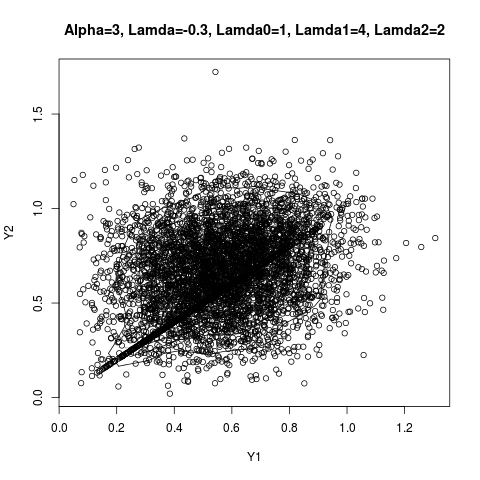
\includegraphics[width=0.90\textwidth]{q2/Question2_1a.png}{\centering}\\
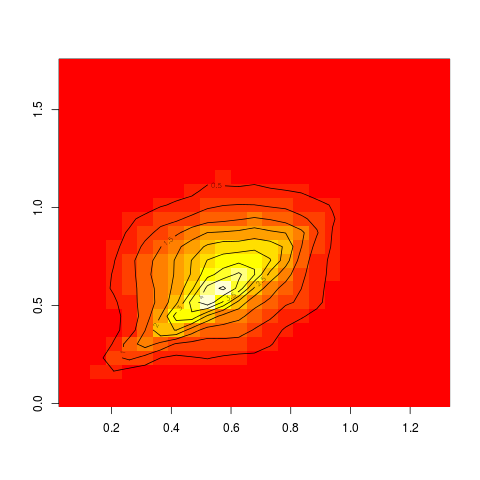
\includegraphics[width=0.90\textwidth]{q2/Question2_1b.png}{\centering}\\
\newpage
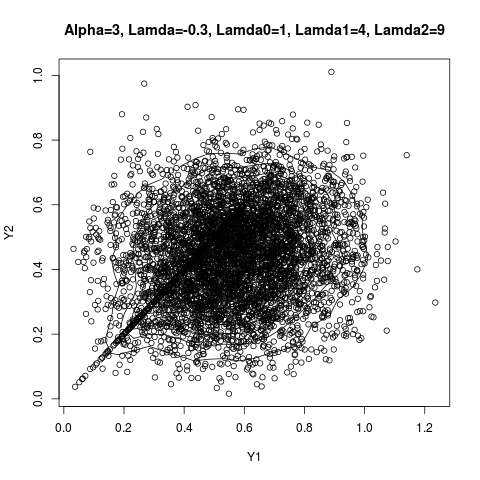
\includegraphics[width=0.90\textwidth]{q2/Question2_2a.png}{\centering}\\
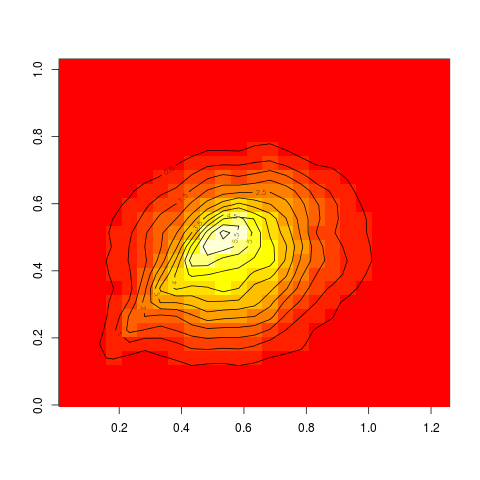
\includegraphics[width=0.90\textwidth]{q2/Question2_2b.png}{\centering}\\
\newpage
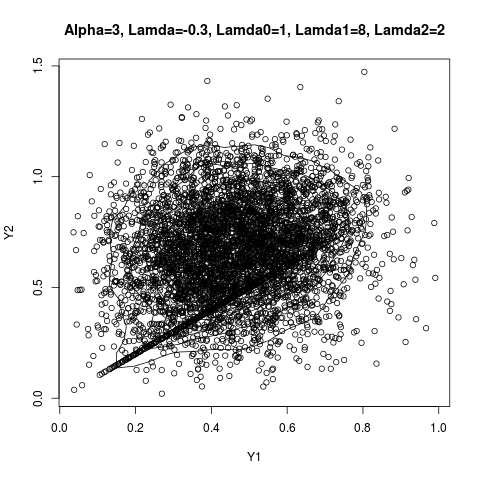
\includegraphics[width=0.90\textwidth]{q2/Question2_3a.png}{\centering}\\
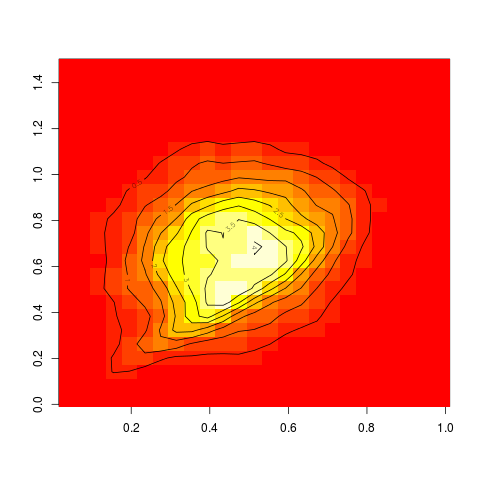
\includegraphics[width=0.90\textwidth]{q2/Question2_3b.png}{\centering}\\
\newpage
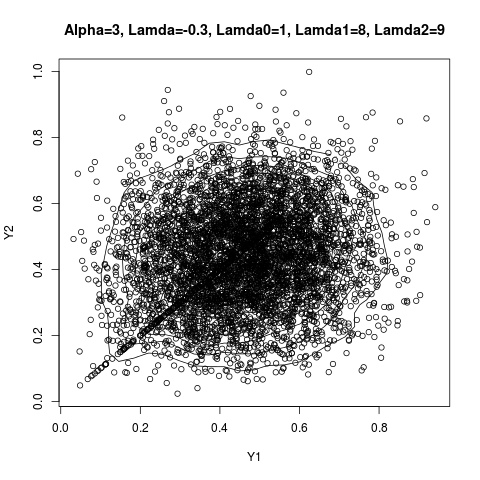
\includegraphics[width=0.90\textwidth]{q2/Question2_4a.png}{\centering}\\
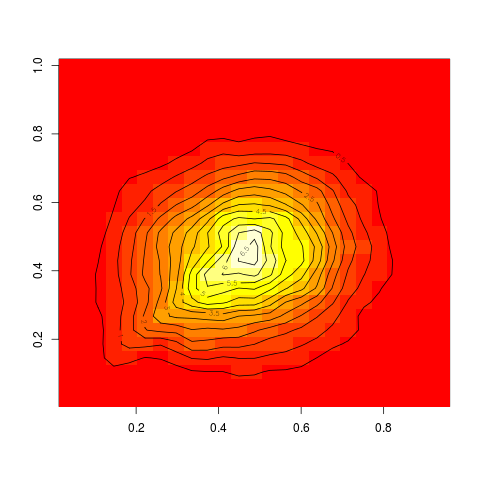
\includegraphics[width=0.90\textwidth]{q2/Question2_4b.png}{\centering}\\
\newpage
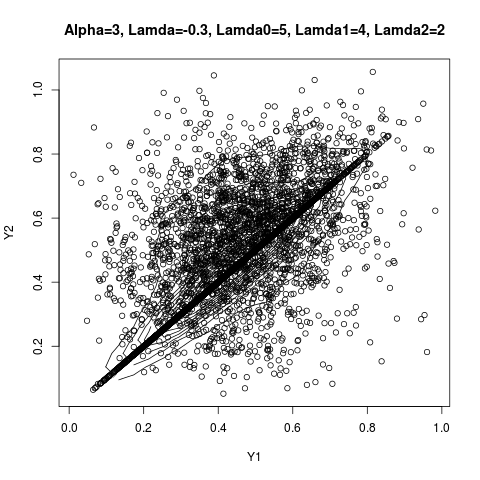
\includegraphics[width=0.90\textwidth]{q2/Question2_5a.png}{\centering}\\
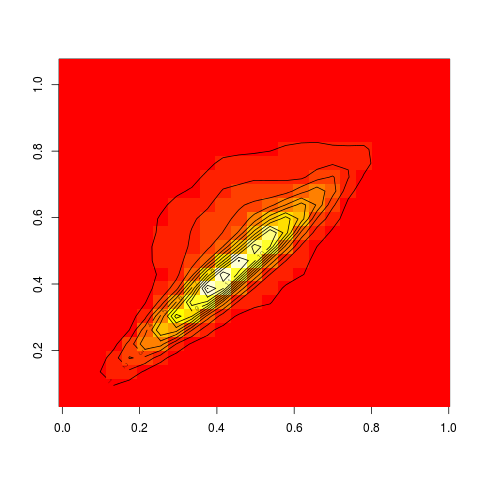
\includegraphics[width=0.90\textwidth]{q2/Question2_5b.png}{\centering}\\
\newpage
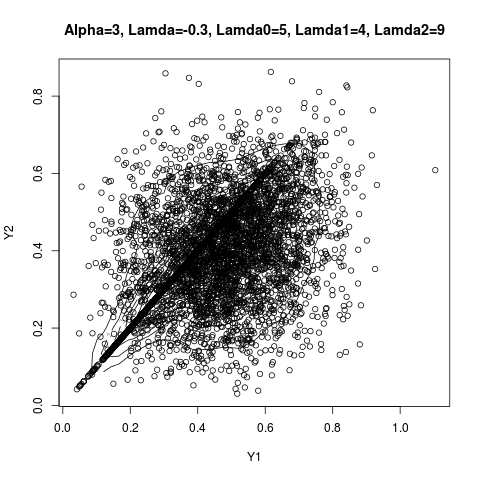
\includegraphics[width=0.90\textwidth]{q2/Question2_6a.png}{\centering}\\
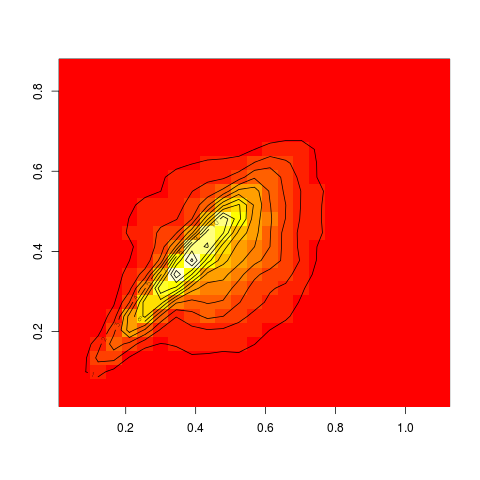
\includegraphics[width=0.90\textwidth]{q2/Question2_6b.png}{\centering}\\
\newpage
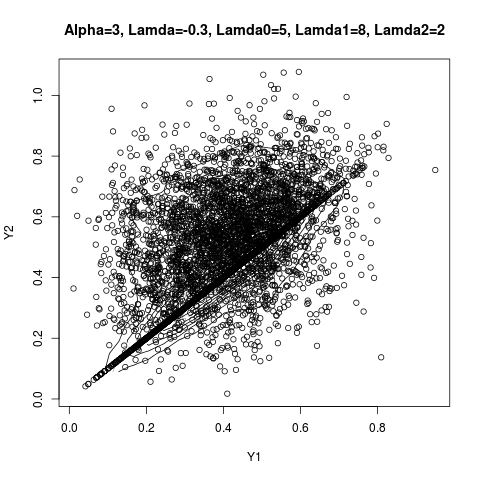
\includegraphics[width=0.90\textwidth]{q2/Question2_7a.png}{\centering}\\
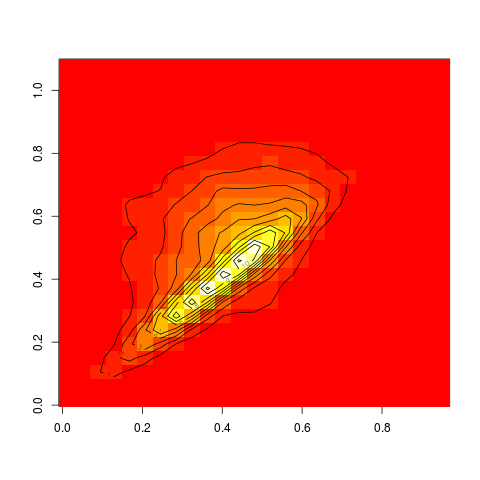
\includegraphics[width=0.90\textwidth]{q2/Question2_7b.png}{\centering}\\
\newpage
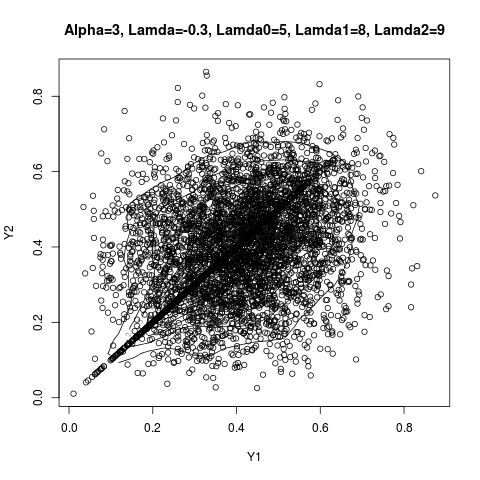
\includegraphics[width=0.90\textwidth]{q2/Question2_8a.png}{\centering}\\
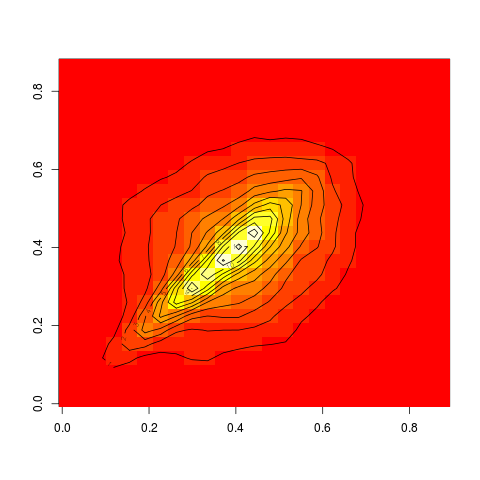
\includegraphics[width=0.90\textwidth]{q2/Question2_8b.png}{\centering}\\
\newpage
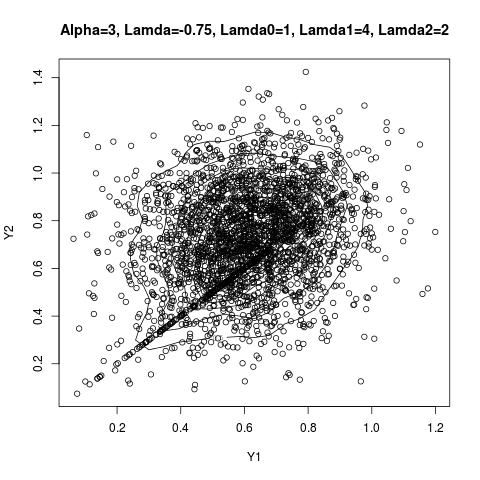
\includegraphics[width=0.90\textwidth]{q2/Question2_9a.png}{\centering}\\
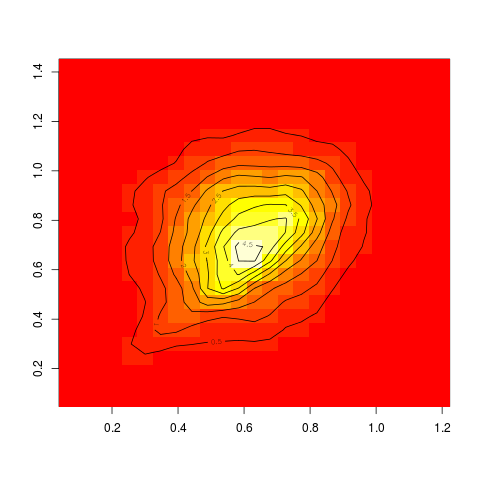
\includegraphics[width=0.90\textwidth]{q2/Question2_9b.png}{\centering}\\
\newpage
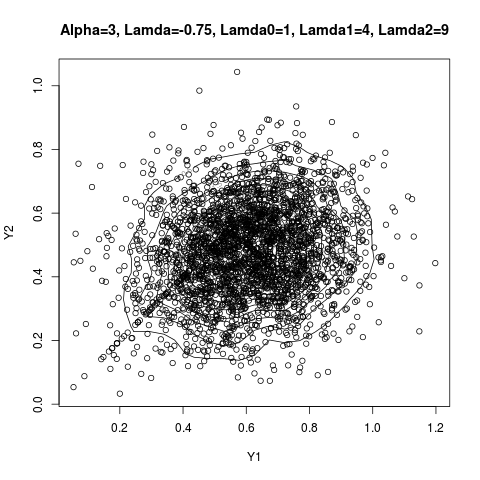
\includegraphics[width=0.90\textwidth]{q2/Question2_10a.png}{\centering}\\
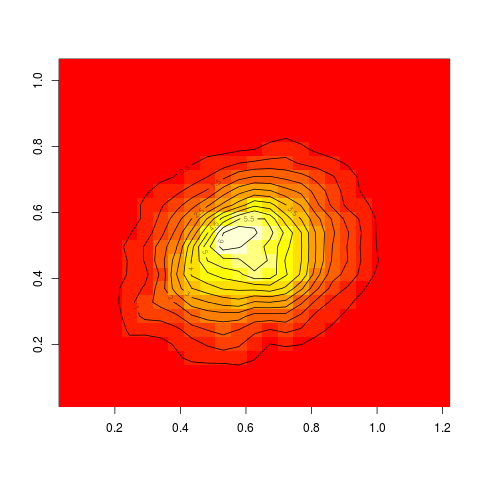
\includegraphics[width=0.90\textwidth]{q2/Question2_10b.png}{\centering}\\
\newpage
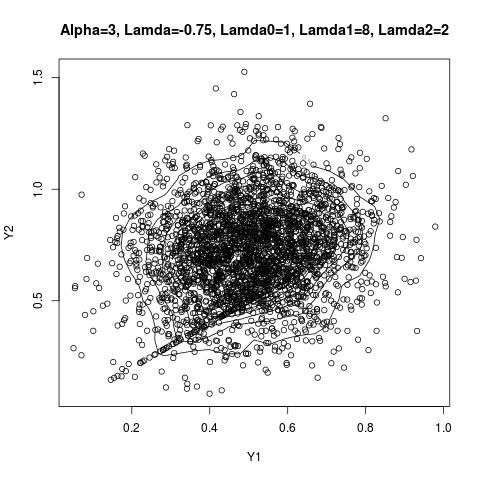
\includegraphics[width=0.90\textwidth]{q2/Question2_11a.png}{\centering}\\
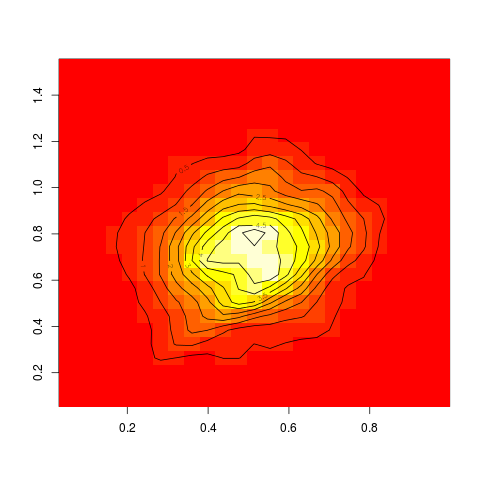
\includegraphics[width=0.90\textwidth]{q2/Question2_11b.png}{\centering}\\
\newpage
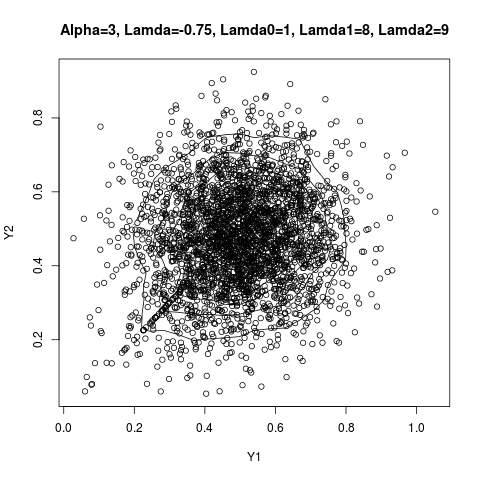
\includegraphics[width=0.90\textwidth]{q2/Question2_12a.png}{\centering}\\
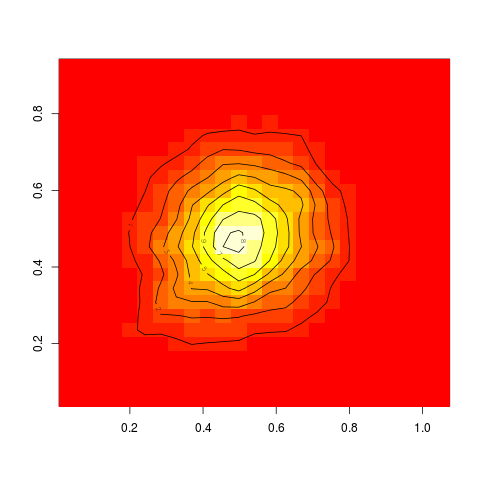
\includegraphics[width=0.90\textwidth]{q2/Question2_12b.png}{\centering}\\
\newpage
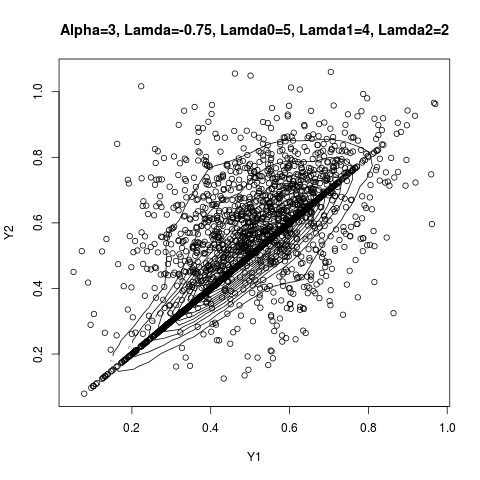
\includegraphics[width=0.90\textwidth]{q2/Question2_13a.png}{\centering}\\
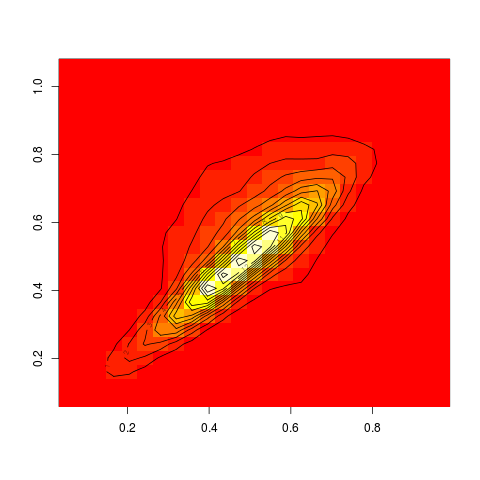
\includegraphics[width=0.90\textwidth]{q2/Question2_13b.png}{\centering}\\
\newpage
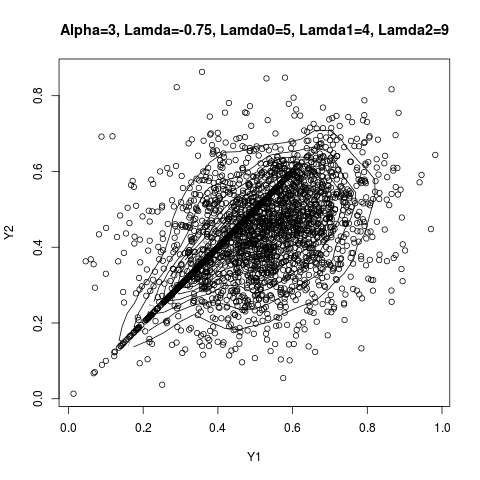
\includegraphics[width=0.90\textwidth]{q2/Question2_14a.png}{\centering}\\
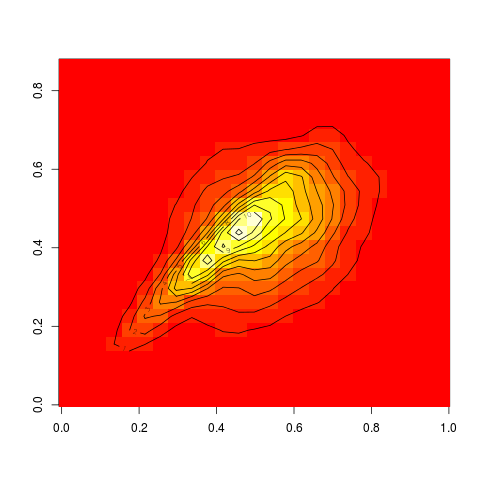
\includegraphics[width=0.90\textwidth]{q2/Question2_14b.png}{\centering}\\
\newpage
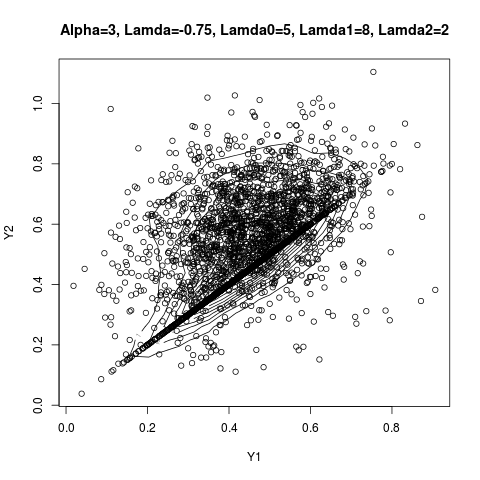
\includegraphics[width=0.90\textwidth]{q2/Question2_15a.png}{\centering}\\
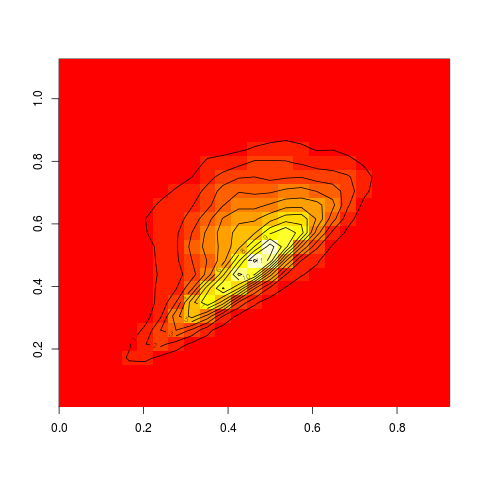
\includegraphics[width=0.90\textwidth]{q2/Question2_15b.png}{\centering}\\
\newpage
\includegraphics[width=0.90\textwidth]{q2/Question2_16a.png}{\centering}\\
\includegraphics[width=0.90\textwidth]{q2/Question2_16b.png}{\centering}\\
\newpage
\includegraphics[width=0.90\textwidth]{q2/Question2_17a.png}{\centering}\\
\includegraphics[width=0.90\textwidth]{q2/Question2_17b.png}{\centering}\\
\newpage
\includegraphics[width=0.90\textwidth]{q2/Question2_18a.png}{\centering}\\
\includegraphics[width=0.90\textwidth]{q2/Question2_18b.png}{\centering}\\
\newpage
\includegraphics[width=0.90\textwidth]{q2/Question2_19a.png}{\centering}\\
\includegraphics[width=0.90\textwidth]{q2/Question2_19b.png}{\centering}\\
\newpage
\includegraphics[width=0.90\textwidth]{q2/Question2_20a.png}{\centering}\\
\includegraphics[width=0.90\textwidth]{q2/Question2_20b.png}{\centering}\\
\newpage
\includegraphics[width=0.90\textwidth]{q2/Question2_21a.png}{\centering}\\
\includegraphics[width=0.90\textwidth]{q2/Question2_21b.png}{\centering}\\
\newpage
\includegraphics[width=0.90\textwidth]{q2/Question2_22a.png}{\centering}\\
\includegraphics[width=0.90\textwidth]{q2/Question2_22b.png}{\centering}\\
\newpage
\includegraphics[width=0.90\textwidth]{q2/Question2_23a.png}{\centering}\\
\includegraphics[width=0.90\textwidth]{q2/Question2_23b.png}{\centering}\\
\newpage
\includegraphics[width=0.90\textwidth]{q2/Question2_24a.png}{\centering}\\
\includegraphics[width=0.90\textwidth]{q2/Question2_24b.png}{\centering}\\
\newpage
\includegraphics[width=0.90\textwidth]{q2/Question2_25a.png}{\centering}\\
\includegraphics[width=0.90\textwidth]{q2/Question2_25b.png}{\centering}\\
\newpage
\includegraphics[width=0.90\textwidth]{q2/Question2_26a.png}{\centering}\\
\includegraphics[width=0.90\textwidth]{q2/Question2_26b.png}{\centering}\\
\newpage
\includegraphics[width=0.90\textwidth]{q2/Question2_27a.png}{\centering}\\
\includegraphics[width=0.90\textwidth]{q2/Question2_27b.png}{\centering}\\
\newpage
\includegraphics[width=0.90\textwidth]{q2/Question2_28a.png}{\centering}\\
\includegraphics[width=0.90\textwidth]{q2/Question2_28b.png}{\centering}\\
\newpage
\includegraphics[width=0.90\textwidth]{q2/Question2_29a.png}{\centering}\\
\includegraphics[width=0.90\textwidth]{q2/Question2_29b.png}{\centering}\\
\newpage
\includegraphics[width=0.90\textwidth]{q2/Question2_30a.png}{\centering}\\
\includegraphics[width=0.90\textwidth]{q2/Question2_30b.png}{\centering}\\
\newpage
\includegraphics[width=0.90\textwidth]{q2/Question2_31a.png}{\centering}\\
\includegraphics[width=0.90\textwidth]{q2/Question2_31b.png}{\centering}\\
\newpage
\includegraphics[width=0.90\textwidth]{q2/Question2_32a.png}{\centering}\\
\includegraphics[width=0.90\textwidth]{q2/Question2_32b.png}{\centering}\\
\newpage
\textbf{MADE BY:\\
Abheek Ghosh 			(140123047)\\
Pawan Vaishnav Madandas (140123048)\\
Divyae Vats             (140123049)\\
Chandan Kumar			(140123050)\\
Prakhaar Bhargava		(140123051)\\}
\end{document} 